% !TEX root = ../thesis.tex

\begin{savequote}[75mm] 
This is some random quote to start off the chapter.
\qauthor{Firstname lastname} 
\end{savequote}

\chapter{Template-based estimation of genome-wide nucleosome positioning via distributed HMC}

%\newthought{Lorem ipsum dolor sit amet}, consectetuer adipiscing elit. Morbi commodo, ipsum sed pharetra gravida, orci magna rhoncus neque, id pulvinar odio lorem non turpis. Nullam sit amet enim. Suspendisse id velit vitae ligula volutpat condimentum. Aliquam erat volutpat. Sed quis velit. Nulla facilisi. Nulla libero. Vivamus pharetra posuere sapien. Nam consectetuer. Sed aliquam, nunc eget euismod ullamcorper, lectus nunc ullamcorper orci, fermentum bibendum enim nibh eget ipsum. Donec porttitor ligula eu dolor. Maecenas vitae nulla consequat libero cursus venenatis. Nam magna enim, accumsan eu, blandit sed, blandit a, eros.

\section{Introduction}
\label{sec:intro}

% General motivation. 
The organization of genetic material within cells plays a major role in the regulation of biological activities.
In the cell, DNA is wrapped around histone proteins to form nucleosomes, which constitute the smallest units of such organization. 
DNA must be accessible for transcription to occur, thus the presence of nucleosomes physically constrains regulation. 
High-throughput sequencing technology produces indirect noisy evidence about the positions of nucleosomes across an entire genome, with an unprecedented resolution.
In this paper, we develop methods to provide accurate, reproducible estimates of nucleosome positions across a genome from high-throughput sequencing data, enabling the investigation of  fine-grained structure in nucleosome positioning and its regulatory role.

% Data, scientific goals and statistical issues
We consider high-throughput sequencing data derived from micrococcal nuclease digestion %, the standard technique in the field
\citep{Tirosh2012}.
% \citep{zawa:moro:broa:2009,Gkikopoulos2011,tolk:zawa:sing:elfv:2011}.
%
Briefly, this technique involves
 linking histone proteins to the target DNA wrapped around them, 
 digesting the remaining DNA using an enzyme,
 then digesting the histone proteins to make the target DNA accessible for further processing \citep[e.g., see][]{Tsankov2010}.
A gel is used to select DNA fragments with an approximate length of 150 base pairs---the length of DNA wrapped around each nucleosome.
These fragments are amplified via PCR and sequenced \citep{Albert2007}.
The resulting sequences, or reads, are aligned to a reference genome for the organism of interest using standard software \citep[Bowtie;][]{lang:trap:pop:salz:2009}.
The data consists of the number of read centers that align to each base pair along the genome.
%
We analyze data obtained with paired-end sequencing technology; that is, each DNA fragment is sequenced simultaneously from both ends, and the two reads are recorded as a pair.
This technology provides the length of each fragment, in addition to its location, following alignment of the paired reads.
Figure \ref{fig:example_data} illustrates some example data.

\ifx\nofigures\undefined
\begin{figure}[b!]
\centering
 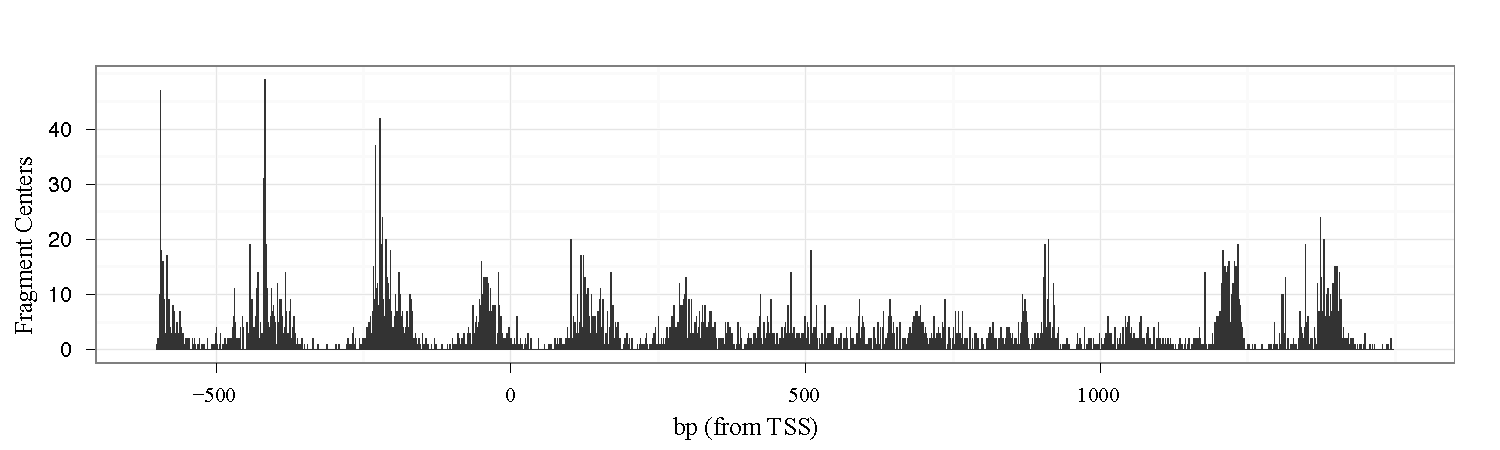
\includegraphics[width=\textwidth]{figures/nucleosomes/readsPlot_H_1-PHO5}
 \caption{Example data for yeast gene PHO5.\label{fig:example_data}} 
\end{figure}
\fi

\subsection{Related work}

%:Related work

\begin{comment}
Separate statistical and biological references.
Incorporate Guillaume's review.
Far less biological detail.
Emphasis on sources of information about digestion variation.
\end{comment}

%The relationship between nucleosome positioning and the regulation of biological activity has been a topic of interest for decades \citep{Albe:John:Lewi:Raff:2002}.
%
The positioning of nucleosomes along the genome was first studied with tiling microarrays \citep{Yuan2005,sega:fond:chen:thas:2006,Lee2007}.
%More recently, tiling arrays have been used to investigate nucleosome movement in yeast \citep{zawa:moro:broa:2009,tolk:zawa:sing:elfv:2011}.
%A comprehensive map of nucleosome positions using tiling arrays is not feasible in organisms with a large genome, since the arrays would have to contain overlapping probes to provide sufficient coverage.
%
High-throughput sequencing data allows for the analysis nucleosome positioning in any organism,
%as it does not rely on probes to quantify the presence of specific cDNA sequences
and overcomes many technical limitations of  tiling microarrays
\citep{Jansen2011}.
%
The first wave of studies using high-throughput sequencing to infer nucleosome positioning used single-end sequencing technology \citep{Albert2007a,Shivaswamy2008,Tsankov2010}.
%\citeauthor{Albert2007a} focused on rotational settings (alternative positioning) in cells at equilibrium, while
%\citeauthor{Shivaswamy2008} focused on the effects of heat shock on transcriptional regulation and chromatin structure.
%\citeauthor{Tsankov2010} instead took a comparative perspective, investigating the relationship between gene expression and chromatin structure across 12 yeast species.
More recent studies have used paired-end sequencing technology \citep{Gkikopoulos2011}.

The statistical approach to identifying nucleosome positions form tiling microarray data consisted largely of hidden Markov models and their variants \citep{Gupta2007,Yuan2008,yass:kapl:jaim:frie:2008,Sun2009a,Mitra2011}, with some mixture model approaches also in use \citep{Sun2009b}.
%
Most analyses of sequencing data have adopted Parzen-window based estimators, which convolve the observed read counts within a window,
extract local maxima, and perform subsequent computations based on taking these maxima as nucleosome positions.
Variants of this technique include the use of multiple windows \citep{Weiner2010}, frequency-based filtering using fast Fourier transformation (FFT) \citep{Flores2011}, and a Kolmogorov-Smirnov based method for detecting differences in nucleosome positioning between samples \citep{Fu2012}.
Others have adapted HMMs to this class of data \citep{Cairns2011}.
%
Model-based analyses of sequencing data have focused on mixture models \citep{Polishko2012,Rashid2011,Zhang2012}.
Recent work combines a new biochemical protocol with a Bayesian deconvolution method \citep{Brogaard2012}; however, their inference procedure targets different estimands.
%% EDO :: BUT .. would be good to state a difference from our approach .. DON'T ACCOUNT FOR DIGESTION VARIABILITY INFORMATION PROVIDED BY THE FRAGMENT LENGTH DISTRIBUTION
% AWB : Not even comparable. It's a completely different biological method with targeted digestion by base pair. They account for their digestion variation, but it's of a completely different type than ours. Fragment length does not provide information for them. Not sure how to say this briefly.

Methodology relevant to the problem we consider has been developed to infer transcription-factor (TF) binding sites from high-throughput ChIP-seq data \citep{park:2009}.
Analyses of ChIP-seq data often combine variants of Parzen window estimation \citep{Schwartzman2011a}, a Poisson model for sequence counts \citep{Zhang2008}, and detection methods for peak finding \citep{Pepke2009}.
%
From a statistical perspective, a key feature of ChIP-seq data is that the TF binding sites are non-overlapping.
This allows for independence assumptions in models for ChIP-seq data \citep{bars:zhao:2009} that cannot be defended in models of nucleosomes, which are likely to overlap when cell populations are sequenced.

%:End of related work

\subsection{Contributions of this article}

% Outline of paper

% Model for paired-end high-throughput sequencing data 
We develop a {\em template-based approach} for estimating the genome-wide distribution of nucleosome positions from paired-end sequencing data.
This approach uses information on fragment lengths provided by paired-end sequencing to estimate the amount of variation due to enzymatic digestion in each lane of sequencing data.
Using this information, we posit a model that captures both the variation of read positions due to enzymatic digestion and the variation due other sources of experimental error, in Section \ref{sec:model}.
This model incorporates a hierarchical structure within discrete segments of the genome to provide local regularization.
We also introduce a set of novel estimands that provide interpretable summaries of the genome-wide distribution of nucleosome positions.

% Inference
%In Section \ref{sec:estimation}, we provide details of inference with this model.
We develop a parallel Hamiltonian Markov Chain Monte Carlo sampler to draw from the posterior distribution of the quantities of interest under our model, in Section \ref{sec:estimation}.
This sampler is highly amenable to distributed computation and scales  linearly with the length of the genome being analyzed.
%Probabilistic inference on the quantities of interest requires estimates of the distribution of digestion errors and the segmentation of the genome.
We provide a non-parametric estimator of the distribution of digestion errors and propose a segmentation algorithm that splits the genome in regions of similar coverage, respecting biological features.
We introduce a calibrated Bayesian method with frequentist error guarantees, to detect local concentrations of nucleosome positions.

% Results and remarks
We demonstrate the proposed methods on real and simulated data in Section \ref{sec:results}, assessing the accuracy and reproducibility of the inferences.
We also compare the performance of our methods to the popular Parzen-window and read-based estimators.
%Each step of this development, from model building through calibrated Bayesian detection and the analysis of reproducibility, is accompanied by decreased reliance on model assumptions and an increase in external validation, ensuring that our method provides robust inferences.
%We conclude with a few remarks on modeling, estimands, and inference in Section \ref{sec:remarks}.

%:End of introduction revisions

\section{Model}
\label{sec:model}

Here we develop a model for paired-end reads, obtained using Solexa high-throughput sequencing technology. 
%
The data consist of integer counts $y_k$ of the fragment centers observed at each base pair $k$ along an $N$-base pair long chromosome, together with the corresponding fragment lengths $l_j$ for each of the $M$ observed fragments, which provide information about how far apart the paired reads are. 
% AWB: Turns out we do need M down in 3.1 (template estimation).

The proposed model consists of two distinct components: an observation model $p(\bm y | \bm \beta)$, which provides the distribution of the observed read counts given the underlying distribution of nucleosome positions $\bm \beta$, and a positioning model $p(\bm \beta | \bm \mu, \bm \sigma^2)$, which describes the structure of the nucleosome position distribution.
%
Given a segmentation function, $\fnDef{s}{\range{1}{N}}{\range{1}{S}}$, which maps the $N$ base pair locations to $S$ regions in which coefficients $\beta_k$ can be assumed to be identically distributed, we posit
\begin{align}
 \label{eq:observation_model}
  y_k|\lambda_k         & \sim \hbox{Poisson } (\lambda_k) \\
 \label{eq:linear_model}
  \bm \lambda_{(N\times 1)} & \equiv X_{(N\times (N - 2 \lfloor \ell_0 / 2 \rfloor))} ~ \bm \beta_{((N - 2 \lfloor \ell_0 / 2 \rfloor)\times 1)}, \\
\nonumber & \quad \beta_k>0 \hbox{ for } k=\lfloor \ell_0 / 2 \rfloor + 1 \dots N - \lfloor \ell_0 / 2 \rfloor \\
\label{eq:positioning_model}
  \log \beta_k        & \sim \hbox{Normal } (\mu_{s_k},\sigma^2_{s_k})
\end{align}
where $X$ specifies the contribution of a nucleosome positioned at base pair $k$ to the expected number of reads at base pair $m$ due to digestion variability, and $s(k)$ is denoted as $s_k$ for compactness.
(The construction of the matrix $X$ is detailed in Section \ref{sec:template}.)
%
The log-likelihood for the proposed model is as follows, subject to the positivity constraint on $\bm \beta$,
\begin{eqnarray}
\label{eq:logLikelihood}
 \log p(\bm y | \bm \theta, \bm \mu, \bm \sigma^2) &=& -\sum_k
\bm x_k^T \bm \beta + \sum_k y_k \log \left( \bm x_k^T \bm \beta \right)  \\
 \nonumber && - \frac{1}{2} \sum_k \log \sigma^2_{s_k} -
  \frac{1}{2} \sum_k \frac{(\theta_k - \mu_{s_k})^2}{\sigma^2_{s_k}}
  + \mathrm{const}.
\end{eqnarray}

To complete the model specifications, we place priors on $\mu_{s}$ and $\sigma^2_{s}$.
We use independent conjugate priors for $\sigma^2_{s}$, assuming $\sigma^2_{s} \sim \mathrm{InvGamma}(\alpha_0, \gamma_0)$.
Our priors for $\mu_{s}$ are fully conjugate and independent across segments; we assume $p(\mu_{s} | \sigma^2_{s}) \sim N(\mu_0, \frac{\sigma^2_{s}}{n_{s} \tau_0})$ where $n_{s}$ is the length of segment $s$.
These stabilize our inferences and reflect vague prior information on the distribution of $\bm \beta$.
This is particularly true for our prior on $\sigma^2_{s}$, which regulates the uniformity of nucleosome positioning.
Their form also allows for efficient computation, as outlined in Section \ref{sec:estimation}.
%
%In practice, we set $\mu_0$ to zero to obtain a simple shrinkage prior. 
%We compared this na\"ive shrinkage strategy with an alternative one, where we
%fix $\mu_0$ at its maximum likelihood estimate  \citep{CloggRubin1991}. 
%In our application, the latter strategy provides no performance gains, while complicating the evaluation of the prior's effect on inferences. 
We analyze the sensitivity of the inferences to the choice of ($\mu_0$,  $\tau_0$, $\alpha_0$, $\gamma_0$) in Section \ref{sec:results}.

% AWB: Tested this idea, and the performance gains are nonexistent. May want to
%		note this, as it strengthens the argument for simple shrinkage

%\subsection{Remarks}
%\label{sec:model_remarks}
%
%The observation model is built around known properties of sample preparation and sequencing, leading to a highly constrained structure among the quantities involved with a direct physical underpinning.  The positioning model is less structured, imposing few assumptions on the details of alternative positioning. This reflects both the lack of prior knowledge in the biology literature and the limited utility of imposing single-cell constraints on a model for cell population measurements.

%%% %%% %%% 

The proposed model depends upon two technical constructs: digestion-variability templates and a  segmentation of the DNA sequence. We discuss them further in the next two subsections, before introducing the estimands of interest in Section \ref{sec:estimands}.

\subsection{Digestion variability template}
\label{sec:template}

A template summarizes variation due to enzymatic digestion in a single lane of sequencing and it is used to build the $X$ matrix in Equation \ref{eq:linear_model}.
We cover the paired-end case here and discuss extensions to single-end sequencing in Section \ref{sec:remarks}.
%
% EDO :: THE PROBABILITY MODEL UNDERLYING THE TEMPLATE WOULD FIND A NATURAL PLACE IN THE PARAGRAPH BELOW. PLEASE DO NOT REMOVE THIS THE TEXT, RATHER COMMENT IT ALL OUT AND REPLACE IT WITH YOUR OWN, SO THAT I CAN TAKE A LOOK AT THE LOGIC AND FLOW BEFORE AND AFTER. 
%
%Technically, $\bm t$ is defined as a function from a finite set of base pairs to $(0,1)$ that specifies the probability of observing a fragment around a given nucleosome location, given that such a fragment originates from the given nucleosome.
%Consider a template that is $2w+1$ base pairs wide, we denote
%the template as a function $t(k) =$ Pr(fragment center is $k$ bp from nucleosome
%location) for $k \in \{-w, \ldots, w\}$. 
%
% AWB edits start
%
Consider a simple model for the variability of enzymatic digestion.
We denote the length of each fragment $j$ as $\ell_j$ and assume
\begin{equation}
\ell_j = \ell_0 + e_{1j} + e_{2j}, \quad e_{1j}, e_{2j} \sim IID \ .
\end{equation}
$\ell_0$ is the base length of each fragment and the $e_{\cdot j}$ terms are the digestion errors at each end of the fragment.
We assume these errors are bounded and symmetric between the ends of each fragment; physically, this means that the enzyme has the same propensity towards over-or under-digestion at each end.
Under this model, each fragment's center varies about its nucleosome's true center according to the distribution of $d_j \equiv \frac{1}{2} (e_{1j} - e_{2j})$.
Our template is this distribution, expressed in vector form and transformed to account for the random rounding of fragment centers to integer positions.
Hence, 
\begin{equation}
t_k = P(d_j = k) + \frac{1}{2}\left( P(d_j = k - \frac{1}{2}) + P(d_j = k + \frac{1}{2}) \right)
\end{equation}
for $k = -w, \dots, w$, yielding a vector $\bm t$ of length $2w + 1$.
We estimate the template from the empirical fragment length distribution corresponding to a lane of paired-end sequencing data, as detailed in Section \ref{sec:templateEstimation}. 
%
% AWB edits end
%
%
Example exact and approximate templates for the same data are shown in Figure \ref{fig:template}.

\ifx\nofigures\undefined
\begin{figure}[t!]
\centering
 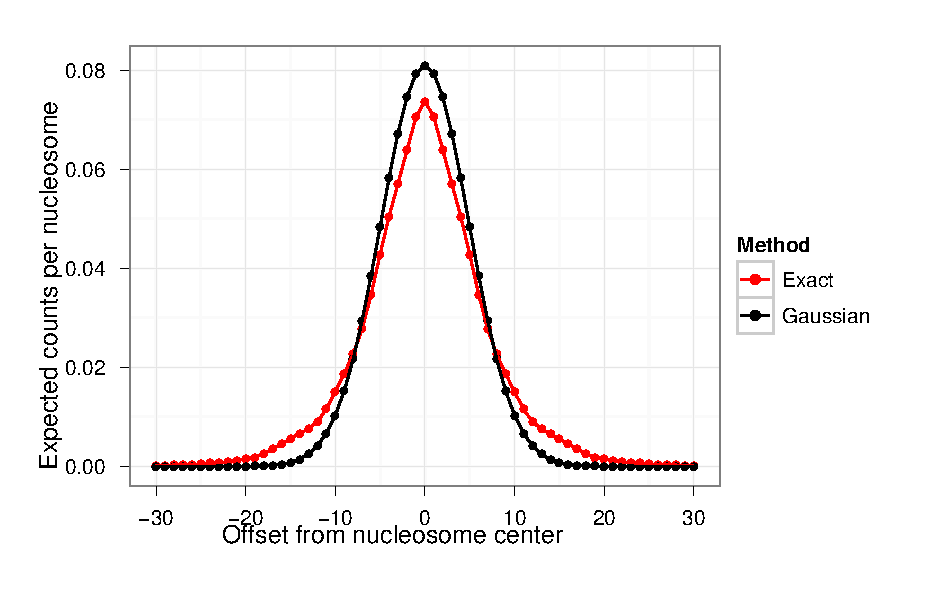
\includegraphics[width=0.8\textwidth]{figures/nucleosomes/plotTemplateVsApprox_H_1-combined}
 \caption{Example templates for yeast growing in high-phosphate.\label{fig:template}} 
\end{figure}
\fi

The matrix $X$ in Equation \ref{eq:linear_model} is constructed using a template $\bm t$ by leveraging an equivalence between a realistic data-generating process and the marginal specification given in Equations \ref{eq:observation_model}--\ref{eq:linear_model}.
%
Briefly, an explicit model would combine a Poisson distribution for the unobservable number of reads that are generated from a given nucleosome location, with a multinomial distribution that controls the offsets of the observed read centers from the center of that nucleosome, which is where they would all be observed in the absence of digestion variability.
%
This Poisson-multinomial structure for the observed reads is marginally equivalent to the more convenient Poisson GLM with an identity link function specified in Equations \ref{eq:observation_model}--\ref{eq:linear_model}.

In detail, denote the length of the sequence of interest $N$, and the width of the template $2w+1$ as above.
%
Then we can define the digestion (or basis) matrix $X$ as an $(N\,\times\,N - \ell_0)$ matrix where each row corresponds to a shifted version of the template.
The matrix $X$ is fully specified as follows,
\begin{equation}
% Aligned vector version
	X = \begin{pmatrix}
	     \bm{t} &&&& \\
	     & \bm{t} &&& \\
	     && \ddots && \\
	     &&& \bm{t} &\\
	     &&&& \bm{t}
	    \end{pmatrix}
\end{equation}
%
Using the $(N - \ell_0)$-dimensional constrained vector of coefficients $\bm
\beta \geq 0$, we obtain an $N$-dimensional vector of expected counts $\bm
\lambda$ using Equation \ref{eq:linear_model}.
%
Each coefficient $\beta_k$ provides the number of fragments we expect to sequence from nucleosomes centered at position $k$.
%
Analogously, $\bm \lambda$ provides the number of fragment centers we expect to observe at each position.
Formally, $\bm \lambda$ is a convolution of $\bm \beta$ with $\bm t$.
This structure models the effect of digestion variability on the observations.

Digestion variability affects the statistical properties of our data in two important ways under this model.
%
First, the expected counts of fragment centers are convolved with the digestion variability template.
This reduces the concentration of counts at each nucleosome position, obscuring the true center of the nucleosome.
%
Second, as digestion variability convolves the expected fragment counts over a broader stretch of the genome, the expected number of counts at each base pair decreases, driving down the signal-to-noise ratio.
This phenomenon is not unique to Poisson noise, but it is particularly acute in this setting because the signal-to-noise ratio of a Poisson random variable is equal to its expectation.
%
The combination of these effects makes inferring nucleosome positions very challenging in this setting, even in high-coverage experiments.
The resulting combination of ``vertical'' noise (from Poisson-lognormal variation) and ``horizontal'' convolution across the sequence (from digestion variability) creates a challenging deconvolution problem.

%%% %%% %%% 

\subsection{Segmentation}
\label{sec:segmentation}

Our segmentation of the DNA sequence accounts for variation in occupancy, coverage, and structure.
%
The goal is to split chromosomes into local regions where the IID assumption on the coefficients $\beta_k$ appear sensible.
The segmentation function $s$ defined above must fulfill a monotonicity condition, $s(k+1)-s(k) \in \{0,1\}$, so that segments are indexed contiguously and in strictly increasing order.
An example segmentation of yeast chromosome I is shown in Figure \ref{fig:segmentation}.
%
\ifx\nofigures\undefined
\begin{figure}[t!]
\centering
 \includegraphics[width=0.8\textwidth]{figures/nucleosomes/plotRegions_H_1-combined_chrom01-small}
 \caption{Example segmentation of yeast chromosome I. See Section \ref{sec:estimation} for estimation details.\label{fig:segmentation}} 
\end{figure}
\fi

Statistically, the segmentation enables local regularization in the estimation of $\bm \beta$.
% 
These coefficients are weakly identified in a model specified by Equations \ref{eq:observation_model}--\ref{eq:linear_model} alone.
Such a model would involve $N - \ell_0$ parameters and $N$ observations, and the Hessian matrix for the implied log-likelihood of $\bm \beta$ would be $H = - X^T W X$, where $W = \diag{y_1 / \bm \lambda_1^2, \ldots, y_n / \bm \lambda_n^2}$.
This is negative-definite if $\bm y$ contains no all-zero subvector of length $2w+1$ or more; otherwise, it is only negative semi-definite.
Furthermore, $H$ is typically very ill-conditioned due to the convolution structure of $X$.
Estimates of $\beta_k$ from this model would be extremely unstable.
%
We regularize the estimates of $\beta_k$ by modeling the distribution of nucleosome positions with Equation \ref{eq:positioning_model}.
In this complete model, we pool information locally within each chromosome, as $\beta_j$ is independent of $\beta_k$ if $s_j \neq s_k$, where $s_k$ is the segment to which base pair $k$ belongs.


Segments divide each chromosome into local stretches over which a consistent distribution of nucleosome positions is plausible.
%
We posit a log-normal distribution for the magnitudes of the coefficients $\beta_k$.
The idea is that most locations on the sequence are expected have a very low concentration of nucleosome positions.
Such locations correspond to small, non-zero values of $\beta_k$.
A few locations have a relatively high concentration of nucleosomes across a population of cells.
These are the positions of interest, corresponding to large values of $\beta_k$.
The log-Normal distribution captures such behavior: it allows the majority of values in $\bm \beta$ to concentrate around a low baseline rate with a few values many orders of magnitude larger than the baseline.
The parameters $\mu_{s_k}$ and $\sigma^2_{s_k}$ control this baseline and the prevalence of extreme values in $\bm \beta$, providing us with a flexible, parsimonious way to regularize our estimation and provide more reliable inferences.

The segmentation also provides a way to control the bias-variance trade-off of our regularization.
Using a large number of short segments results in low bias, as they can capture sequence features at a fine scale; however, this also leads to greater uncertainty, as more parameters are introduced and less observations are available for regularization within each segment.
Using a smaller number of longer segments produces the opposite effect.
We discuss a strategy to managing this trade-off in Section \ref{sec:segmentationAlgorithm}.


\subsection{Estimands}
\label{sec:estimands}

We can express the scientific estimands of interest as functions of $\bm \beta$.
The parameter $\bm \beta$ itself is of interest, as it captures the pattern of nucleosome positioning across each chromosome. However, $\bm \beta$ is  high-dimensional and unsuitable for human interpretation. 
The posterior expectation, standard deviation, and quantiles of $\bm \beta$ are useful for visualization and exploratory analysis.
Below, we develop several more refined estimands to quantify the structure of the nucleosome position distribution.
These new estimands fall into two broad categories:
 (1) local measures of concentration, and
 (2) cluster-level summaries of structure.

The first family of estimands aims to quantify the relative concentration of nucleosome centers within a local window.
Formally, for each base pair location $k$ in $\bm \beta$, we consider the ratio
\begin{equation}
C_{p,l}(k) = \frac{\sum_{i=-p}^{p} \beta_{k + i}}{\sum_{i=-l}^{l} \beta_{l + i}} \label{eq:concentration} \ ,
\end{equation}
where $2l + 1$ is the width of a local window and $2p + 1$ is the width of the region of interest.
We typically choose $l = 73$, yielding a local window of width 147.
%
For $l \leq 73$, the structure of $\bm \beta$ within $2l+1$ bp windows can be taken as measure of the distribution of nucleosome positions across the population of cells.
Physically, a nucleosome consists of 147bp of DNA wrapped around histone proteins, so, within a single cell, nucleosomes must be spaced by at least 147bp.
As a result, each cell can contribute at most one nucleosome center within a window of width 147bp or less.
Thus, the relative magnitudes of the entries of $\bm \beta$ within such a window reflect only the distribution of nucleosome positions across cells, not the arrangement of multiple nucleosomes within any individual cell.
% EDO :: THIS COMMENT IS UNCLEAR. MY GUESS IS THAT EITHER IT'S THE OPPOSITE, OR WE CAN NEVER TAKE A LOCAL CONCENTRATION MEASURE AS A SINGLE-CELL QUANTITY. EITHER WAY, OR IF I AM WRONG, PLS REVISE FOR CLARITY. I CANNOT TELL ..
% AWB: Revised and expanded. Core idea is that each cell can only contribute a single nucleosome within a small window due to physical spacing constraints.

Choosing $p = 0$ yields a measure of relative concentration at each base pair in the chromosome.
However, choosing $p > 0$ is generally preferred to account for biological variation in nucleosome positions.
These estimands come with a useful baseline.
Assuming a uniform local distribution of nucleosome positions across cells in the population would imply $C_{p,l}(k) = \frac{p}{l}$.
Deviations from this baseline provide a normalized measure of local concentration.
We present strategies for the detection of local nucleosome concentrations based on these estimands in Section \ref{sec:detection}.

The second family of estimands provides summaries of small clusters of nucleosome positions.
By definition, these estimands rely on a procedure to identify local clusters, such as Parzen window filtering, applied to the estimated vector of $\bm \beta$ coefficients.
Because of this, these estimands may inherit issues from this clustering procedures; however, they are useful for comparative analysis and can capture interesting patterns.
We define the estimand $\bm \kappa$ to be the cluster centers obtained by running the selected clustering method on $\bm \beta$.
$\bm \kappa$ is a cluster-level estimand itself, but it is primarily of interest as a means to obtain summaries of $\bm \beta$ within individual clusters.
We consider
%a measure of local occupancy, obtained by summing the entries of $\bm \beta$ contained within each cluster, and a measure of
measures of structure, localization, and sparsity within the cluster, defined as the normalized entropy, mean absolute deviation, and quantiles of the entries of $\bm \beta$, taken as an unnormalized discrete distribution over the base pairs in the cluster.
Formally, considering cluster $\bm \beta_{[i:j]}$ and defining $p_{[i,j]}(k) = \beta_k / \sum_{m=i}^{j} \beta_m$, our localization, structure, and sparsity measures are defined as
\begin{eqnarray}
L_{i,j} &=&  1 - \frac{4}{j - i + 1} \sum_{k=i}^{j} p_{[i,j]}(k) |k - m_{i,j}|, \, m_{i,j} = \sum_{k=i}^{j} k p_{[i,j]}(k) \label{eq:localization} \\
S_{i,j} &=&  1 + \frac{1}{\log(j - i + 1)} \sum_{k=i}^{j} \log p_{[i,j]}(k) \label{eq:structure} \\
R_{i,j,q} &=& 1 - \frac{n_{i,j,q} - 1}{q (j - i + 1)}, \, n_{i,j,q} = \min\left(n : \sum_{k=i}^{i + n} \tilde{p}_{[i,j]}(k) \right) \label{eq:sparsity} \ ,
\end{eqnarray}
respectively, where $\tilde{p}_{[i,j]}(k)$ is $p_{[i,j]}(k)$ sorted in descending order.
All measures are normalized so $L_{i,j} = S_{i,j} = R_{i,j,q} = 0$ if $\bm \beta_{[i:j]}$ is constant and $L_{i,j} = S_{i,j} = R_{i,j,q} = 1$ if $\bm \beta_{[i:j]}$ contains only one non-zero entry.
%These estimands measure provide interpretable measures of local structure.

Using the methods described in Section \ref{sec:estimation}, we can obtain draws from the posterior distribution of all of these estimands.
This allows us to cleanly separate the modeling of the measurement process and broad properties of nucleosome positioning from the features of interest.

\section{Inference, estimation, and computation}
\label{sec:estimation}

To extract useful inferences from the model of Section \ref{sec:model}, we must address three sets of unknown quantities: the digestion template $\bm t$, the segmentation of each chromosome $s$, and the parameters and latent variables of the positioning model, $\bm \beta$, $\bm \mu$, and $\bm \sigma^2$.
The parameter $\bm \beta$ and quantities derived from it are of the greatest scientific interest, as they correspond directly to the chromatin structure.
However, before inferring $\bm \beta$, we address $\bm t$ and $s$.

To estimate the template $t$ from paired-end sequencing data, we develop a non-parametric method, in Section \ref{sec:templateEstimation}.
We develop a simple algorithm to segment each chromosome into non-overlapping segments with useful biological and statistical properties, in Section \ref{sec:segmentationAlgorithm}.
%
Using the estimated template $t$ and segmentation $s$, we turn to model-based inference for $(\bm \beta, \bm \mu, \bm \sigma^2)$.
We build a parallel MCMC algorithm that can efficiently sample from the joint posterior of these parameters,  in Section \ref{sec:mcmc}.
By combining the conditional independence structure of our model with distributed computation, we are able to handle datasets where $\bm \beta$ contains millions of entries.

An approximate EM algorithm is also provided in the online supplement %[\cite{supplementInference}]
as an optional initialization step for this sampling.
The EM approach provides a computationally-efficient way to obtain rough estimates of these parameters, but the joint posterior distribution of $(\bm \beta, \bm \mu, \bm \sigma^2)$ has a complex multimodal structure that EM is ill-equipped to address.
Implementation details are given in the online supplement. % [\cite{supplementInference}].

Finally, we calibrate the frequentist operating characteristics of our Bayesian estimators using a permutation null hypothesis, detailed in Section \ref{sec:detection}.
This ensures that our conclusions are valid both as Bayesian posterior probability assessments and under frequentist criteria.
We focus on controlling the false discovery rate (FDR) for the detection of local structure in the distribution of nucleosome positions.

\subsection{Template estimation}
\label{sec:templateEstimation}

Recall from Section \ref{sec:template} that we model the length of each fragment as $ l_j = l_0 + e_{1,j} + e_{2,j} $.
We assume that $e_{1,j}$ and $e_{2,j}$ (the digestion errors) are independent and identically distributed, and $l_0$ is fixed at $147$, which is the known length of DNA wrapped around a single nucleosome.
We show how $e_{1,j}$ and $e_{2,j}$ relate to each fragment in Figure \ref{fig:digestErrors}.
Along the genome, the distributions of digestion errors at the ends of each fragment are mirror images of each other, so positive values imply that some DNA not bound to a nucleosome is under-digested, so $l_j > l_0$.

To setup our estimation problem, we define two probability distributions,
\begin{eqnarray}
 p(i) &=& Pr \left( l_j = i \right) \\
 q(i) &=& Pr \left( e_{1,j} = i \right).
\end{eqnarray}
Physically, $l_j \geq0$, which implies $e_{1,j}, e_{2,j} \geq - \lfloor \frac{l_0}{2} \rfloor$. Analogously, if the longest observed fragment length is
$l_{max}$, we have  $Pr \left( l_j > l_{max} \right) = 0$. We require $l_j\leq l_{max}$, which imples $e_{1,j}, e_{2,j} \leq l_{max} - l_0 + \lfloor \frac{l_0}{2} \rfloor$. Thus, we can write 
\begin{equation}
 p(i) = \sum_{k=-\lfloor \frac{l_0}{2} \rfloor}^{l_{max} - l_0 + \lfloor
\frac{l_0}{2} \rfloor} q(k) q(i - l_0 - k).
\end{equation}

\ifx\nofigures\undefined
\begin{figure}
\centering
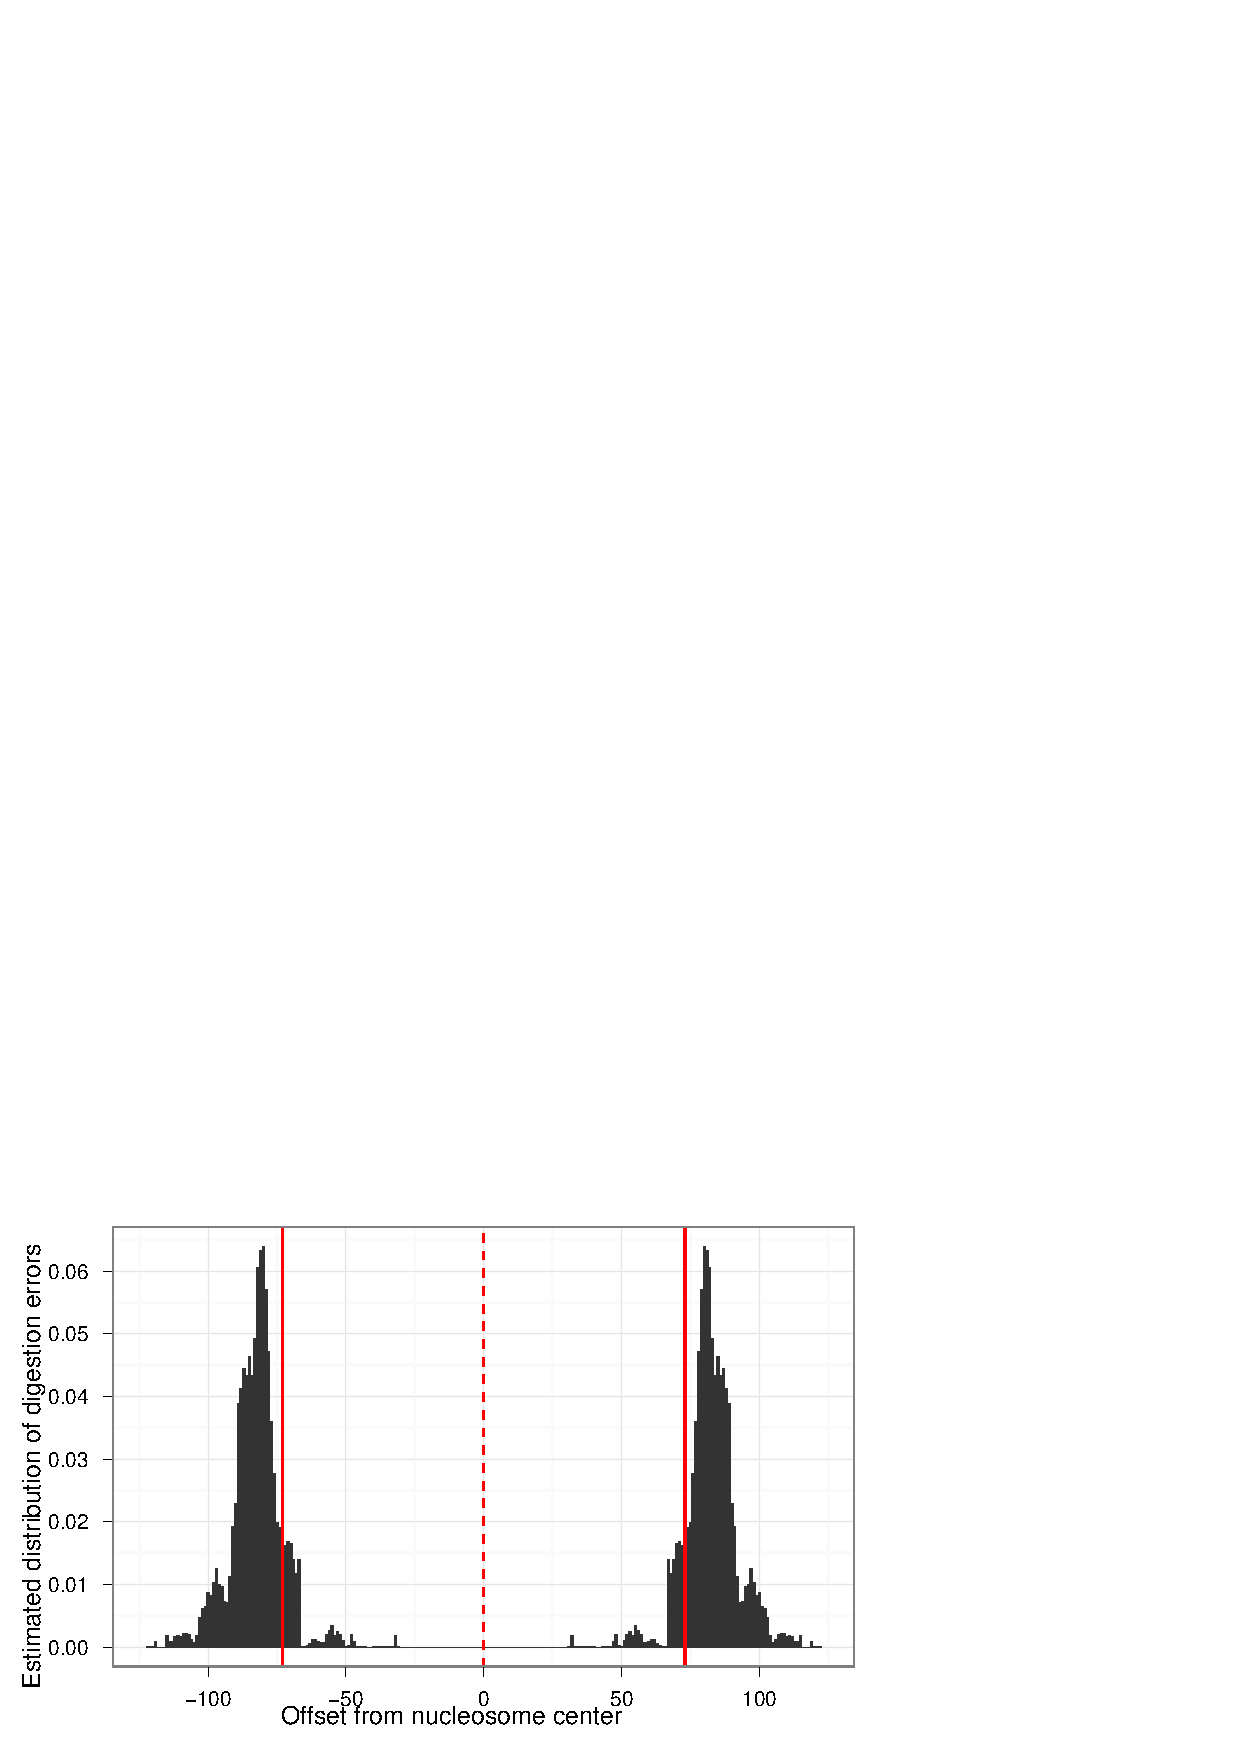
\includegraphics[width=0.75\textwidth]{figures/nucleosomes/plotDigestionDist_histogram}
\caption{Estimated digestion error distributions vs. offset from nucleosome
center; vertical lines at $\pm \l_0 / 2$ (solid) and nucleosome center (dashed).
\label{fig:digestErrors}}
\end{figure}
\fi

The resulting log-likelihood for the observed fragment lengths is $\sum_{j = 1}^{M} \log p(l_j)$.
We maximize this numerically, using a multivariate logit transformation on the values of $q(k)$ to avoid bounded optimization.
Using the L-BFGS-B algorithm \citep{lbfgsb1997} on a laptop with a Core i5 processor and 8GB of RAM, this maximization requires approximately 40 seconds for a typical experiment.
This computation scales only with the number of unique fragment lengths observed, so it cannot become bottleneck for this method.

We obtain the template distribution $t$ from $q$ via a convolution sum and  linear transformation.
Recall from Section \ref{sec:template} that $t$ is the distribution of $\frac{e_1-e_2}{2}$, restricted to the integers via random rounding.
We first obtain the distribution of $e_1-e_2$ via
\begin{equation}
 u(i) = P(e_1-e_2=i) = \sum_{k=-\lfloor \frac{l_0}{2} \rfloor}^{
 l_{max} - l_0 + \lfloor \frac{l_0}{2} \rfloor}
 q(k) q(k-i) \ .
\end{equation}
We finally transform the distribution $u(i)$ to the desired template $t(i)$ by accounting for random rounding, as
\begin{equation}
 t(k) = \frac{1}{2}u(2k-1) + u(2k) + \frac{1}{2}u(2k+1) \ .
\end{equation}
%The same random rounding procedure is used to map fragment centers to a single location on the genome.
Thus, the estimated template accurately reflects both the variation due to enzymatic digestion and the details of our preprocessing.
We use this estimated template to build the design matrix $X$ in the observation model, as discussed in Section \ref{sec:model}, and for the simulation study discussed in Section \ref{sec:design}.

\subsection{Segmentation algorithm}
\label{sec:segmentationAlgorithm}

% Hierarchical merging with coverage
We estimate the segmentation function $\fnDef{s}{\range{1}{N}}{\range{1}{S}}$ by leveraging the biological structure of each chromosome.
We begin by enumerating all open reading frames (ORFs) and intergenic regions on a given chromosome.
Merging overlapping ORFs into single segments yields a starting set of contiguous, non-overlapping segments.
Many of these segments are too short to provide useful local regularization.
To increase the segmentation's utility, we merge neighboring segments until all segments exceed a minimal length (800bp for the purposes of the analysis in Section \ref{sec:results}).

We iteratively merge the most similar short segments until the resulting segmentation fulfills the given minimum length constraint.
We measure similarity using the coverage within each segment, defined as
\begin{equation}
 c_i = \frac{1}{n_i} \sum_{k \,:\, s(k)=i} y_k \ ,
\end{equation}
where $n_i$ is the length of segment $i$.
Algorithm \ref{alg:segmentation} provides pseudocode for this procedure.

\begin{algorithm}
  \textbf{Given} Minimum segment length $M$; initial segmentation\;
  Calculate $\{n_i\}$ and $\{c_i\}$\;
  \While{$\min_i n_i < M$}{
    Clear minimal difference in coverages $d_m$ and index $i_m$\;
    \tcc{Find the best merge among short segments}
    \For{$i \,:\, n_i < M$}{
      Compute $d_i = \min( |c_i - c_{i-1}|, |c_i - c_{i+1}| )$\;
      \If{ $d_i < d_m$ }{
        Update $d_m = d_i$ and $i_m = i$\;
      }
    }
    \tcc{Execute best merge}
    Merge segment $i_m$ with neighbor having nearest coverage\;
    Update $\{n_i\}$ and $\{c_i\}$\;
  }
  \Return{Segmentation $s$}
  \medskip
  \caption{Segmentation algorithm \label{alg:segmentation}}
\end{algorithm}

At the conclusion of Algorithm \ref{alg:segmentation}, we obtain a segmentation for which each segment has enough observations to provide useful local regularization.
The boundaries of each segment also align with biologically-meaningful features, as every step in the above procedure maintains segment boundaries as a subset of ORF boundaries.
% TODO: Revisit
This estimated segmentation is fixed and used in all subsequent inference.

\subsection{Posterior sampler}
\label{sec:mcmc}

The MCMC sampler consists of two alternating updates.
At each iteration $r$, our algorithm
%% EDO :: T IS ALSO THE NOTATION FOR THE TEMPLATE, I DON'T FIND THIS PARTICULARLY DISTURBING, SINCE NOW T (TEMPLATE) IS GONE AND SUBSUMED INTO X (BASIS MATRIX), BUT I THOUGHT I'D MAKE A NOTE OF THIS.
% AWB: Changed from t to r. Don't think that conflicts with any other notation.
\begin{enumerate}
 \item Draws $(\bm \mu^{(r)}, \bm \sigma^{2\,(r)}) | \bm \beta^{(r-1)}$ directly, then
 \item Updates $\bm \beta^{(r)} | (\bm \mu^{(r)}, \bm \sigma^{2\,(r)})$ via a distributed HMC step.
\end{enumerate}
The first update is straightforward as we can directly sample from the conditional posterior of $(\bm \mu^{(t)}, \bm \sigma^{2\,(t)})$.
This is a standard conjugate normal update, given the log-normal hierarchical structure, and operates independently across segments.
We give details in the online supplement. % [\cite{supplementInference}].

The second update is computationally challenging.
The chromosomes of S. cerevisiae range in length from 230,218 to 1,531,933 base pairs, so the $\bm \beta$ vectors are very high-dimensional.
In some of the experiments discussed in Section \ref{sec:results}, we work with simulated chromosomes with over 3.85 million base pairs.
%% EDO :: AGAIN HERE base pairs IS WITHOUT HYPHEN AND WITH A SPACE. ANYTHING GOES, AS LONG AS IT IS CONSISTENT THROUGHOUT THE PAPER -- I PREFER base-pairs IN CASE YOU ARE WONDERING
The conditional posterior of $\bm \beta^{(t)} | (\bm \mu^{(t)}, \bm \sigma^{2\,(t)})$ is not part of any standard family, so we turn to Hamiltonian Monte Carlo (HMC).
The dimensionality of $\bm \beta$ makes a single HMC update for the entire vector both computationally infeasible and numerically unstable.
To enable fast, statistically-efficient computation, we take advantage of the conditional independence structure of this conditional posterior.

Subvectors of $\bm \beta$ separated by at least $2w$ entries are conditionally independent given $(\bm \mu^{(t)}, \bm \sigma^{2\,(t)})$ and the entries of $\bm \beta$ between them.
Consider the subvectors $\bm \beta_{[j_1 : j_2]}$ and $\bm \beta_{[k_1 : k_2]}$, with $j_1 < j_2 < k_1 < k_2$.
The elements of $\bm \beta_{[j_1 : j_2]}$ affect only $\bm \lambda_{[j_1 - w : j_2 + w]}$, and the elements of $\bm \beta_{[k_1 : k_2]}$ affect only $\bm \lambda_{[k_1 - w : k_2 + w]}$.
Hence, if $k_1 > j_2 + 2w$, then $\bm \beta_{[j_1 : j_2]}$ and $\bm \beta_{[k_1 : k_2]}$ are conditionally independent given $\bm \mu$ and $\bm \sigma^2$.

We take advantage of this conditional independence to construct a distributed set of HMC updates.
We first fix the length of each subvector that will be updated via a single HMC step to $B > 4w$.
Next, consider two partitions of $\bm \beta$ into subvectors.
The first starts at the beginning of $\bm \beta$ and proceeds forward with subvectors of length at most $B$ separated by $2w$, yielding
$$\bm \beta_{[1 : B]}, \bm \beta_{[B + 2w + 1 : 2B + 2w]}, \ldots, \bm \beta_{[n_b (B + 2w) + 1 : N]} \ .$$
The second begins at the $B/2$th entry of $\bm \beta$ and again proceeds forward in subvectors of length at most $B$, as
$$\bm \beta_{[B/2 + 1 : 3B/2]}, \bm \beta_{[3B/2 + 2w + 1 : 5B/2 + 2w]}, \ldots, \bm \beta_{[n_b (B + 2w) B/2 + 1 : N]} \ .$$
Within each partition, the subvectors are conditionally independent, and, in combination, these partitions include all entries of $\bm \beta$.

Within each iteration of our sampler, we cycle through each of these partitions, updating each subvector of $\bm \beta$ with one HMC step.
As each subvector within each parition is conditionally independent, we can execute all HMC steps in parallel for each partition.
This allows us to distribute the computational burden over hundreds of cores, providing fast scalable inference.
Each of these distributed HMC steps is, on its own, relatively standard.
However, they are much faster than expected, as the log-conditional posterior's value and gradient can both be computed via a convolution, lowering the computational cost per core to $O(B \log B)$ with the fast Fourier transform. 
%% EDO :: WE DON'T NEED THE FFT ACRONYM IF WE USE THIS ONLY ONCE, OR IF WE USE IT LATER SPELL IT OUT THE FIRST TIME. ALSO, IT IS NOT IMMEDIATELY CLEAR TO ME HOW THE FFT IS USED IN THIS CONTEXT, PERHAPS A SENTENCE WOULD HELP.
% AWB: See sentence below.
In particular, all matrix-vector products involving the $X$ matrix can be computed as convolutions with the template vector $\bm t$ instead, reducing the complexity of such products from $O(B^2)$ to $O(B \log B)$.
Details of distributed algorithm, computational infrastructure, and tuning of the HMC are given in the online supplement. % [\cite{supplementInference}].
A Python implementation of the sampler is available on GitHub, \url{www.github.com/awblocker/cplate}	
%% EDO :: PROVIDE THE URL
% AWB: Done. Repository is currently private.

\subsection{Detection and calibration}
\label{sec:detection}

Recall from Section \ref{sec:estimands} that we quantify  local concentrations of nucleosomes using the estimand $C_{p,l}(k)$, which defines local concentrations as small regions of the chromosome that contain a density of nucleosomes greater than that we would expect under a uniform distribution of nucleosomes across cells in our population, $p / l$.
%% EDO :: PLS MAKE THIS ESTIMAND CAPITAL C THROUGHOUT, FOR CONSISTENCY WITH THE OTHER TWO ESTIMADS; ALSO AVOID CONFLICTS WITH COVERAGE STATISTICS WE USED TO ESTIMATE THE SEGMENTATION
% AWB: Done

We can estimate $P(C_{p,l}(k) > p / l \mid \bm y)$ for each base pair $k$ using the MCMC sampler described in Section \ref{sec:estimation}.
However, we require greater security in our detection results than the Bayesian approach alone can provide.
To quantify the operating characteristics of our procedure and provide frequentist guarantees on its performance, we turn to a permutation null.

Our null hypothesis is that $\bm y$ consists of a set of multinomial draws.
Under this null, the entries of $\bm y$ within each segment $i$ are drawn from a multinomial distribution with equal probability assigned to each base pair within the segment and $n = \sum_{k : s(k) = i} y_{k}$.
This null hypothesis rests on the same idea as Fisher's exact test: we condition on the marginal distribution of the data and consider all independent permutations of the observations. 
We approximate this null distribution by repeatedly randomly permuting the observed reads within each segment.

We then run our MCMC sampler on each such draw from the null, using the template and segmentation estimated from the observed data.
From the sampler's output, we obtain an estimate of the distribution of $P(C_{p,l}(k) > p / l | \bm y)$ over positions $k$ under the null.
We compare this to the distribution of posterior probabilities for the observed data and set a detection threshold to control the FDR using the method of \citet{StoreyTibshirani2003}.
For example, with the datasets analyzed in Section \ref{sec:results}, we have typically found that a threshold of approximately $0.8$ on $P(C_{p,l}(k) > p / l | \bm y)$ yields a FDR of 5\% or less.
This approach provides a secure detection procedure with both Bayesian and frequentist interpretations.


\section{Results}
\label{sec:results}

We demonstrate the proposed methods on  real and simulated data.
%
High-throughput sequencing data were collected on S. cerevisiae cell populations growing in a high-phosphate medium.
The data consist of two lanes of sequencing, referred to as technical replicates, on each of two separate samples with different enzymatic digestion, referred to as biological replicates.
Analyses with the proposed methods are highly reproducible, as we show in Section \ref{sec:reproducibility}, and provide new insights on the fine-grained structure of nucleosome positioning.
The biological relevance of these substantive findings is detailed elsewhere \citep{Xu:Alex:Edo:Erin:2011}.

The simulation studies aim to demonstrate the utility of the estimands introduced in Section \ref{sec:estimands} used in combination with the proposed deconvolution approach to inference, as well as the scalability of our methods.
In Section \ref{sec:design}, we describe the design of the simulation studies. 
We simulate high-throughput sequencing data with different coverage, on genes with primary and alternative nucleosome positions, with different degrees of variation throughout the population. 
In Section \ref{sec:mcmcPerformance}, we discuss the efficiency and scalability of inference via parallel Hamiltonian Markov Chain Monte Carlo sampling.
In Section \ref{sec:clusterPower}, we compare the performance of the proposed method to that of a Parzen-window estimator followed by greedy search \citep[the standard in the field;][]{Albert2007,Shivaswamy2008,Tsankov2010,Tirosh2012} for estimating measures of structure, quantifying power and error in estimating the locations of clusters of nucleosome positions.
In Section \ref{sec:localPower}, we assess the performance of the proposed method for estimating measures of local concentration, quantifying power and error in estimating the locations of distinct primary and alternative positions.
%
In both Sections \ref{sec:clusterPower} and \ref{sec:localPower}, we use design-based analysis of variance (ANOVA) to quantify the relative contributions to estimation errors of coverage, distance between primary and alternative positions and their relative frequencies across the cell population.
We also use logistic regression to analyze the sensitivity of power to the three experimental factors we consider.
% AWB: Where did all of the stability across populations come from? That's not in our simulations. Also, do precisely evaluate discrimination between primaries and alternatives. It's location estimation for both.
%
In Section \ref{sec:reproducibility}, we assess the reproducibility of our inferences for cluster-level summaries of nucleosome positioning (Section \ref{sec:clusterReproducibility}) and the locations of local concentrations (Section \ref{sec:detectionReproducibility}).
We also compare the reproducibility of our cluster-level inferences to those obtained from Parzen-window methods and read-based estimators of the cluster-level estimands.

To perform inference throughout this section, we set $\mu_0 = 0$, $\tau_0 = 1/10$, $\alpha_0 = 7$, and $\gamma_0 = 10$.
These values were chosen to be weakly-informative on the basis of prior biological information.
These values of $\alpha_0$ and $\gamma_0$ imply that there is a 99\% prior probability that 0.2--13\% of base pairs have $\beta_k$ greater than or equal to 10 times their median.
%
We found little sensitivity of our inferences to these choices of parameter values, using data from chromosome I.
For instance, sweeping $\tau_0$ over two orders of magnitude (0.01--1) showed little effect on inferences, as did similar changes to $(\alpha_0, \gamma_0)$.

\subsection{Experimental design}
\label{sec:design}

To assess the performance of the proposed methods, we generated  artificial chromosomes using the classical principles of experimental design.
These artificial chromosomes consist of a series of genes, each containing a set of nucleosome positions.
We fix the length of each gene to 3501bp, consisting of a 1000bp promoter region, of a 2500bp coding region, and of a 1bp transcription start site (TSS).

We designed a simulation with three factors, varied at the gene level: coverage (the expected number of reads per gene), the spacing between primary nucleosome positions and alternative positions (which we refer to as offset), and the relative magnitudes of  primary and alternative positions.
Coverage had 10 levels, spanning the 5th to 95th percentile observed gene-level coverages in increments of 10\%.
Alternative position spacing had 10 levels, spanning from 0bp (no alternative positions) to 45bp in increments of 5bp.
Alternative position magnitude had 11 levels, spanning from 0 (no alternative positions) to 1 (alternative positions of the same magnitude as primary positions) in increments of 0.1.
Thus, the effective magnitude of the primary position relative to the alternative positions ranged from 1 to $\frac{1}{3}$.
We used a full factorial design on these three factors, yielding 1100 distinct treatments for each of 10 simulated chromosomes.
%
We then constructed a realistic distribution of nucleosome positions within each artificial gene.
Using one of our high-phosphate data sets, we first identified clusters of nucleosome positions using the standard Parzen window method.
We indexed these clusters by their ordering within each actual gene, considering 1000bp before TSS to the end of each ORF, and computed the proportion of reads within the ORF observed within each such cluster.
Finally, we averaged over the positions and proportions of these clusters by their order from their TSS, obtaining the average offset from the TSS and relative occupancy of the first, second, third, etc. clusters before and after the TSS.
Figure \ref{fig:repgene} provides an illustration of both coefficients, $\beta_k$, and read counts $y_k$, for one gene.

\ifx\nofigures\undefined
\begin{figure}
\begin{center}
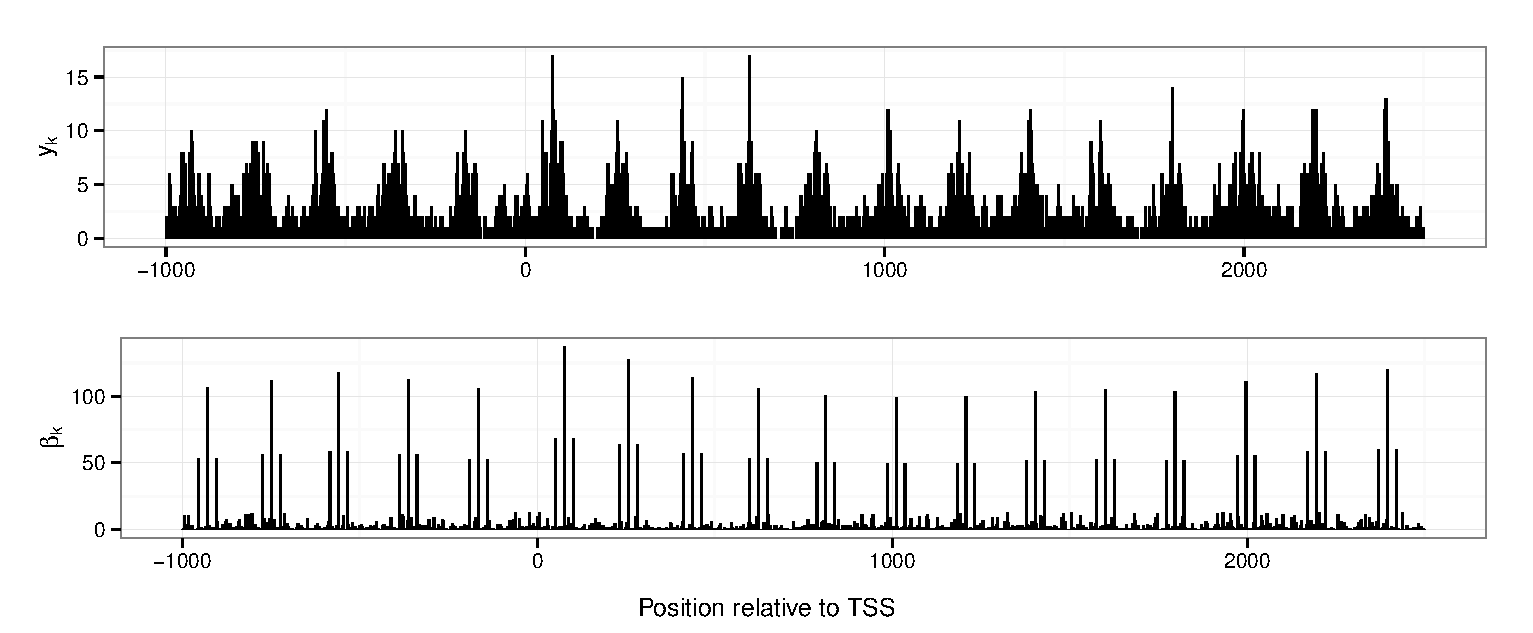
\includegraphics[width=\textwidth]{figures/nucleosomes/plot_repGene_combined}
\caption{Illustration of one simulated gene: $0.55$ quantile of coverage, with alternative position magnitude of $0.5$, and alternative positions at $\pm 25$bp from each primary position. Read counts $y_k$ (top panel), and coefficients $\beta_k$ (bottom panel). \label{fig:repgene}}
\end{center}
\end{figure}
\fi

To generate our artificial dataset, we followed a modified version of the generative process outlined in Section \ref{sec:model}.
For each gene, we first drew coefficients for its subset of $\bm \beta$ from an upper-truncated log-normal distributed with parameters estimated from those regions with similar coverage.
These are our ``background'' positions.
Then, we set the entries of $\bm \beta$ corresponding to the gene's primary and alternative positions deterministically.
The sum of the coefficients for these positions was fixed to the remaining total occupancy of the gene, less the sum of the background positions.
Their relative magnitudes were determined by the design described above, with two alternative positions placed symmetrically around each primary position at the designated spacings.
Thus, for a given level of coverage, the expected number of reads within each cluster was fixed, but its distribution across primary and alternative positions varies.

We convolved these $\bm \beta$ vectors with the template estimated from the experimental data to obtain vectors of expected read counts $\bm \lambda$.
Finally, we generated $\bm y \sim \mathrm{iid} \Poisson(\bm \lambda)$ to obtain simulated read counts.
This entire procedure was repeated for each replicate, yielding 10 artificial chromosomes of length 3,851,100bp each.

These simulations are inspired by our generative model, but they do not follow it's structure to the letter.
The distribution of background coefficients and the effects of digestion agree between our model and our simulations.
However, we introduce much more structure into the locations of nucleosome concentration via the deterministic placement of primary and alternative positions.
This simultaneously provides a stringent test of our methods and decreases the amount of residual variation across our experimental replicates.
As a ``sanity check'' on this design, simulated read counts were shown side-by-side with matched actual read counts to experienced biologists in this field.
They could not reliably distinguish between the simulated and actual data.
We provide further algorithmic details for this procedure and supporting figures in the online supplement. % [\cite{supplementSim}].

\subsection{Parallel HMC performance}
\label{sec:mcmcPerformance}

The parallel Hamiltonian Monte Carlo sampler performed well on both real and simulated datasets, based on standard MCMC diagnostics.
For the actual and simulated datasets used in Section \ref{sec:results}, we ran 2,000 iterations, discarding the first 200 as burn-in.
This yielded 1,800 draws for $\bm \beta$, $\bm \mu$, and $\bm \sigma^2$.
The mean effective sample size for the elements of $\bm \theta = \log \bm \beta$ in the real dataset was 1573, with 99\% of the coefficients having effective sample sizes between 304 and 2057.
For the simulated dataset, the mean was 1675 with 99\% between 520 and 2011.
Gelman-Rubin diagnostics based a set of MCMC runs with dispersed initializations on the smallest chromosome (I) showed multivariate potential scale reductions of 1.05 or less.

Our sampler proved extremely scalable.
Using 144 cores on the Harvard Odyssey cluster and setting $B = 2000$, each simulated chromosome required 1.83 seconds per iteration for a total runtime of approximately 1 hour.
The smallest S. cerevisiae chromosome (I) required 0.136 seconds per iteration, while the largest (IV) required 0.699 second per iteration, yielding total runtimes of 4.5 and 23.3 minutes, respectively.
Running the entire S. cerevisiae genome required approximately 3.24 hours.
The sampler was also run on an Amazon EC2 cluster with 512 cores, processing the same genome in under an hour.

\subsection{Power analysis}
\label{sec:power}

Using simulated chromosomes, we compare the performance of the proposed method to that of a Parzen-window estimator for estimating locations of clusters of nucleosome positions, and assess the performance of the proposed methods for detecting and estimating the locations of both primary and alternative positions.
For both analyses, we use ANOVA to quantify the relative contributions to estimation errors of coverage, distance between primary and secondary positions and their relative frequencies across the cell population.
We complement these with logistic regression to analyze the sensitivity of power to these three experimental factors.

The ground truth consists of the primary and alternative positions generated in Section \ref{sec:design}, along with their coefficients.
Recall that the output of the calibrated detection procedure, detailed in Section \ref{sec:detection}, is a series of positions where high local concentrations have been detected, and the output of  the cluster-based estimands is a series of cluster centers.
%
% EDO :: in section estimands we talk about measures of "local concentration" and "local structure". It would be nice to keep that language throughout, rather than talking about "cluster-based estimands" and "smaller-scale structure". As of now, I myself keep on getting confused about which is which. Certainly don't expect a non-interested reviewer too keep up. Let's discuss and make the language consistent. I stopped modifying from here on, but some way to connect the two would be helpful at this point. I did what I could to keep the distinction straight.
%
To assess performance in estimating cluster positions, we match inferred cluster centers to ground truth cluster centers.
Similarly, to assess performance of local concentration measures, we match detected local concentrations all ground truth positions, primary and alternative.
%
Finding the nearest estimated position for each ground truth position yields measures of power, as we can measure the distance from each true position to the nearest inferred one.
Large distances imply low sensitivity, and vice versa.
Conversely, finding the nearest ground truth position for each inferred position yields measures of accuracy.
If inferred positions are far from the true ones, we would consider the results unreliable.

The analyses below are based on summaries of these matched distances; we compute mean and median absolute errors, and we tabulate the proportion of true positions matched to an inferred positions within a fixed number of base pairs.
The first set of quantities summarize distributions of errors in estimated positions, while the second is directly interpretable as a measure of power.

\subsubsection{Clusters}
\label{sec:clusterPower}

Detection of a cluster was defined as a best-match distance of less than 5bp between the inferred and true cluster center ($\kappa_m$).
Figure \ref{fig:powerCluster} summarizes our key findings, showing the relative power of each method against the effective magnitude of the primary position, the offset of the alternative positions, and gene-level coverage.
Tables \ref{tab:clusterAnova} provides the results of a design-based ANOVA of the mean absolute errors of  estimated cluster locations, by gene, and Table \ref{tab:clusterGlm} provides the results of a logistic regression of power on the design factors.
%
\ifx\nofigures\undefined
\begin{figure}
\centering
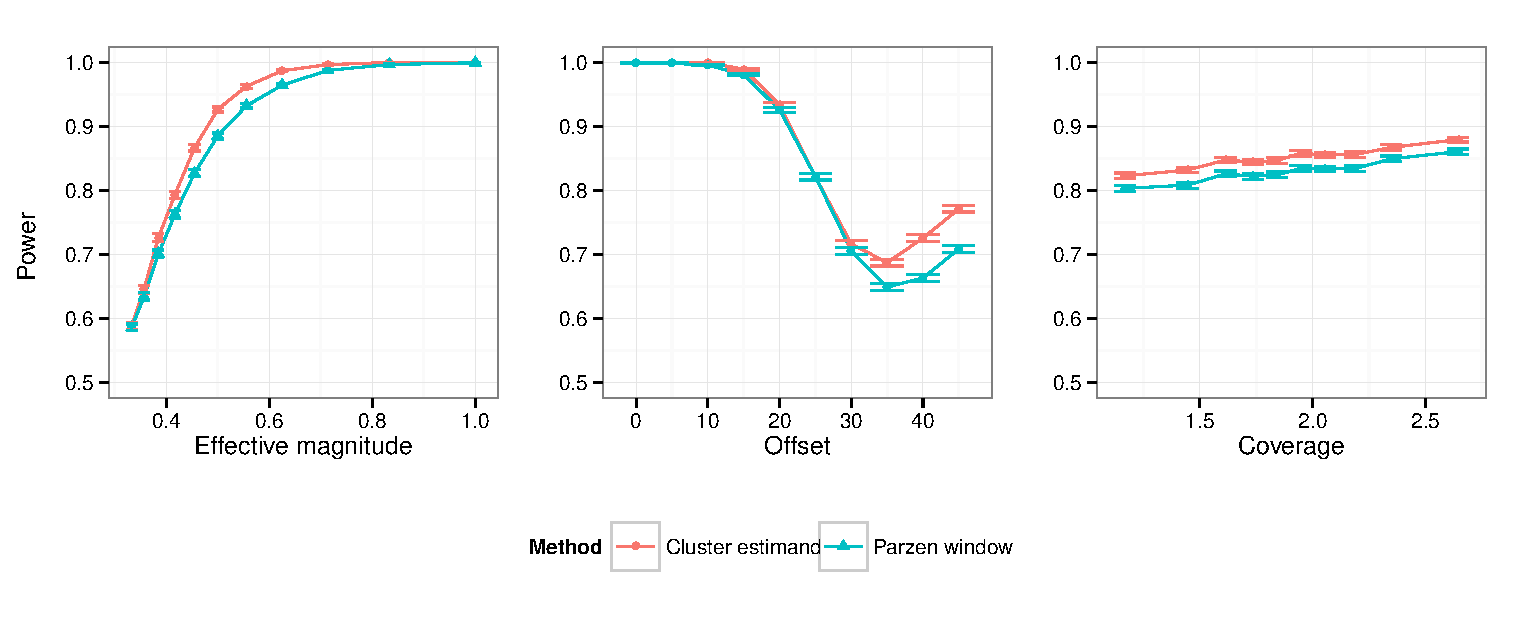
\includegraphics[width=\textwidth]{figures/nucleosomes/figure_power_cluster_3-panel}
\caption{Power vs. effective magnitude (left), alternative position offset (center), and coverage (right) for Parzen window and cluster estimand methods \label{fig:powerCluster}}
\end{figure}
%
\begin{table}
\centering{}%
\begin{tabular}{lr|rr|rr}
\hline 
 &  & \multicolumn{2}{c|}{Cluster Estimand} & \multicolumn{2}{c}{Parzen Window}\tabularnewline
\hline 
 & Df  & Sum Sq  & F value  & Sum Sq  & F value \tabularnewline
\hline 
Coverage & 9  & 1928.94  & 198.73  & 753.24  & 79.04 \tabularnewline
Offset  & 9  & 19422.58  & 2001.01  & 10789.06  & 1132.10 \tabularnewline
Magnitude  & 9  & 10764.55  & 1109.02 & 6768.51  & 710.22 \tabularnewline
Coverage:Offset  & 81  & 275.41  & 3.15 & 264.68  & 3.09 \tabularnewline
Coverage:Magnitude  & 81  & 175.19  & 2.01 & 142.80  & 1.66 \tabularnewline
Offset:Magnitude  & 72  & 23535.40  & 303.09 & 19172.33  & 251.47 \tabularnewline
Coverage:Offset:Magnitude  & 648  & 950.25  & 1.36  & 947.80  & 1.38 \tabularnewline
Residuals  & 10090  & 10881.93  &  & 10684.31  & \tabularnewline
\hline 
\end{tabular}\caption{Analysis of variance of absolute errors in cluster centers for cluster
estimand and Parzen window methods. All factors and interactions were
statistically significant with $p<0.0001$.
\label{tab:clusterAnova}}
\end{table}
%
\begin{table}[ht]
\centering{}%
\begin{tabular}{r|rr|rr}
\hline 
 & \multicolumn{2}{c|}{Cluster Estimand} & \multicolumn{2}{c}{Parzen Window}\tabularnewline
\hline 
 & Estimate  & z value  & Estimate  & z value \tabularnewline
\hline 
(Intercept)  & 3.3461  & 54.15  & 3.4660  & 56.74 \tabularnewline
Coverage & 0.6069  & 5.20  & 0.7498  & 6.54 \tabularnewline
Offset  & -5.3115  & -58.00  & -5.4596  & -60.92 \tabularnewline
Effective Magnitude  & 2.7211  & 10.76  & 2.3296  & 10.82 \tabularnewline
Coverage$\cdot$Offset  & -0.4217  & -2.48  & -0.6071  & -3.66 \tabularnewline
Coverage$\cdot$Effective Magnitude  & 1.7927  & 3.20  & 0.9037  & 2.02 \tabularnewline
Offset$\cdot$Effective Magnitude  & 8.9842  & 22.27  & 6.9932  & 21.15 \tabularnewline
Coverage$\cdot$Offset$\cdot$Effective Magnitude  & 2.1476  & 2.52  & 1.8962  & 2.84 \tabularnewline
\hline 
\end{tabular}\caption{Logistic regression of power on design factors as continuous variables
cluster estimand and Parzen Window method. Are regressors are normalized
to have range $[0,1]$.
\label{tab:clusterGlm}}
\end{table}
\fi
%
For estimating cluster locations, the proposed method dominates the Parzen-window estimator both in terms of power, with average difference of 2.1\%, and mean absolute error (not shown) across all conditions.
Power ranges from approximately $12\%$ to $100\%$ over all factor combinations in our experiments for both methods, while mean absolute position errors range from approximately 0.1 to 60bp.
Our method provided an average power of 85\%, while the Parzen window method's average power was 83\%.
Power shows a strong dependence on the local distribution of nucleosome positions; the accuracy in identifying the cluster centers of primary positions is reduced by the presence of stable alternative positions.
The spacing between primary and alternative positions also affects power substantially, with power diminishing by approximately 30\% as the offset increase from 0 to 35bp.
Power increases slightly for both methods at offsets of 40 and 45bp.
The relative performance of the proposed method is largest for offsets over 30bp, with a difference in power of 7\% at 45bp.
Power shows little marginal dependence upon local coverage with only a 6\% change in power over the range of coverages for both methods.

The ANOVA and logistic regression analyses support these observations and provide further insights into the role of interactions between the design factors.
ANOVA results in Table \ref{tab:clusterAnova} indicate that alternative position offset, effective magnitude, and their interaction account for the vast majority of variation in absolute position errors (approximately 75\% of total variation and 94\% of explained variation) for both methods.
Logistic regression results in Table \ref{tab:clusterGlm} suggest that the power of the proposed method and of the Parzen window estimator respond similarly to the experimental factors.
The marginal effects of offset and effective magnitude are strongly negative and positve, respectively, but the offset-effective magnitude interaction effect is overwhelmingly large and positive.
Coverage has a weak marginal effect on power, but it enters more strongly in the interaction with effective magnitude and in the three-way interaction.

Taken together, these results demonstrate that the proposed method offers improved performance relative to the standard method in the field, for estimating cluster locations.
However, the proposed method offers the greatest benefits for exploring  local concentration in the distribution of nucleosome positions, an estimand that the Parzen-window estimator cannot reliably infer.

\subsubsection{Local concentrations}
\label{sec:localPower}

We next examine the ability of the proposed method to detect local concentrations in the distribution of nucleosome positions, a quantification of small-scale structure.
We focus on detecting small regions of excess local concentration using the $C_{p,l}(k)$ estimand, defined in Equation \ref{eq:concentration}.
For this analysis, we fix $l = 73$ and $p = 3$, and used the calibrated detection procedure described in Section \ref{sec:detection} with a maximum FDR of 5\%.\footnote{We reduce any contiguous sequences of detections to their mean position for interpretability. This is conservative in terms of FDR control and provides a more stringent test of the proposed methodology.}
%
For primary positions, we declare a successful detection if the best-match distance is less than 5bp between a detected position and the true primary position.
For alternative positions, we declare a successful detection if the best-match distance between a detected position and the true alternative position is less than $1/2$ of the alternative position's distance from its primary position.
%
Figure \ref{fig:powerLocal} summarizes our results for primary and alternative positions, showing the power of the proposed method against the effective magnitude of the primary position, the offset of the alternative positions, and gene-level coverage.
Tables \ref{tab:detectionAnova} provides the results of a design-based ANOVA of the mean absolute errors of  estimated cluster locations, by gene, and Table \ref{tab:detectionGlm} provides the results of a logistic regression of power on the design factors.
%
\ifx\nofigures\undefined
\begin{figure}
\centering
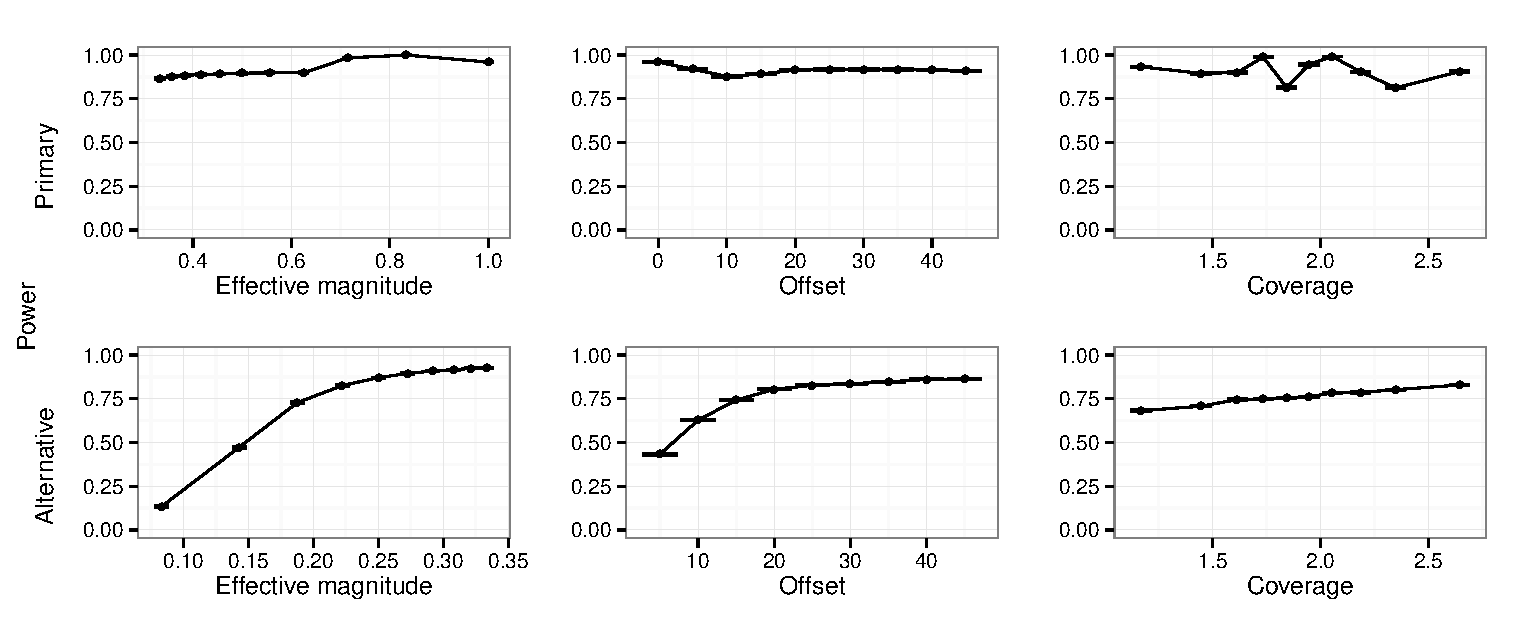
\includegraphics[width=\textwidth]{figures/nucleosomes/figure_power_combined-pm3_3-panel}
\caption{Power vs. effective magnitude (left), alternative position offset (center), and coverage (right) for detection of primary and alternative positions $\pm 3$bp \label{fig:powerLocal}}
\end{figure}

\begin{table}[t!]
\centering{}%
\begin{tabular}{l|rrr|rrr}
\hline 
 & \multicolumn{3}{c|}{Primary Positions} & \multicolumn{3}{c}{Alternative Positions}\tabularnewline
\hline 
 & Df  & Sum Sq  & F value  & Df  & Sum Sq  & F value \tabularnewline
\hline 
Coverage & 9  & 1453.02  & 63.02{*} & 9  & 11136.04  & 1825.67{*} \tabularnewline
Offset  & 9  & 5837.60  & 253.20{*}  & 8  & 34614.74  & 6384.17{*} \tabularnewline
Magnitude  & 9  & 116496.93  & 5052.88{*}  & 9  & 74825.85  & 12267.12{*} \tabularnewline
Coverage:Offset  & 81  & 147.78  & 0.71\phantom{*}  & 72  & 5331.20  & 109.25{*} \tabularnewline
Coverage:Magnitude  & 81  & 1292.48  & 6.23{*}  & 81  & 4532.05  & 82.55{*} \tabularnewline
Offset:Magnitude  & 72  & 2964.07  & 16.07{*} & 72  & 154557.47  & 3167.31{*} \tabularnewline
Coverage:Offset:Magnitude  & 648  & 1043.81  & 0.63\phantom{*}  & 648  & 3968.16  & 9.04{*} \tabularnewline
Residuals  & 10090  & 25847.85  &  & 8100  & 5489.74  & \tabularnewline
\hline 
\end{tabular}\caption{Analysis of variance of absolute position errors for the detection
of primary and alternative positions using local concentration estimands.
{*} indicates that a factor was statistically significant with $p<0.0001$.
Remaining factors had $p$-values larger than 0.95.
\label{tab:detectionAnova}}
\end{table}
%
\begin{table}[t!]
\centering{}%
\begin{tabular}{r|rr|rr}
\hline 
 & \multicolumn{2}{c|}{Primary Positions} & \multicolumn{2}{c}{Alternative Positions}\tabularnewline
\hline 
 & Estimate  & z value  & Estimate  & z value \tabularnewline
\hline 
(Intercept)  & 1.7018  & 2.13  & -1.6631  & -44.64 \tabularnewline
Coverage & -0.0456  & 2.33  & 0.4591  & 7.12 \tabularnewline
Offset  & 0.4778  & 0.82  & -1.5089  & -20.65 \tabularnewline
Effective Magnitude  & 2.0866  & 14.07  & 2.1086  & 38.37 \tabularnewline
Coverage$\cdot$Offset  & -0.5585  & -1.42  & 1.0953  & 8.64 \tabularnewline
Coverage$\cdot$Effective Magnitude  & -0.7448  & -5.31  & -0.3608  & -3.75 \tabularnewline
Offset$\cdot$Effective Magnitude  & 0.9623  & 2.62  & 7.8374  & 55.50 \tabularnewline
Coverage$\cdot$Offset$\cdot$Effective Magnitude  & -0.3217  & -0.95  & 8.7109  & 31.84 \tabularnewline
\hline 
\end{tabular}\caption{Logistic regression of power on design factors as continuous variables
for primary and alternative positions. Are regressors are normalized
to have range $[0,1]$.
\label{tab:detectionGlm}}
\end{table}
\fi

Power ranges from approximately 64\% to 100\% for primary positions and from approximately 2\% to 100\% for alternative positions across all combinations of factors, while mean absolute position errors range from 0.389 to 6.61bp and from 2.17 to 41.8bp, respectively.
The sensitivity of power and absolute position errors to the experimental factors differs between primary and alternative positions.

For primary positions, the power increases as the effective magnitude of the primary position increases and decreases as the offset to the alternative position increases.
The ANOVA results in Table \ref{tab:detectionAnova} suggest that the majority of variation in absolute estimation errors for primary positions (75\% of total and 90\% of explained) is driven by the relative magnitude of primary and alternative positions.
Coverage plays a minor role in the variation of these errors, even when including all of its interactions.
The logistic regression results in Table \ref{tab:detectionGlm} tell a similar story, with effective magnitude of the primary position and its interaction with the offset to the alternative position showing a strong positive effect on power.
Other effects are considerably smaller.

For alternative positions, the power increases as effective magnitude of the primary position, the offset to the alternative position, and the coverage increase.
The ANOVA results in Table \ref{tab:detectionAnova} show that the majority of the variation in absolute estimation errors for alternative positions is accounted for by the offset-magnitude interaction (52\% of total, 53\% of explained), with the marginal contributions of magnitude, offset, and coverage accounting for most of the remaining variation (41\% of total, 42\% of explained).

The logistic regression results in Table \ref{tab:detectionGlm} support these findings and shed more light on the drivers of power for primary and alternative positions.
The marginal effect of effective magnitude of the primary position is similar for primary and alternative positions, but the offset-effective magnitude and three-way interactions are far stronger for alternative positions than they are for primary positions.
Coverage also has a pronounced effect on power for alternative positions, both marginally and through the interaction terms.

Taken together, these results demonstrate that the proposed method can detect local concentrations in the distribution of nucleosome positions across a broad range of realistic conditions.
We can reliably detect and estimate the locations primary positions with average power over 90\% and average absolute position errors of only 2.1bp.
Although alternative positions are more difficult to detect, the proposed method provides reliable inferences about their positions as well, yielding an average power of 76\% and mean absolute position errors of 6.0bp.
% AWB: Compelling wrap-up in 2 sentences; statement of victory...
We discuss the implications of these capabilities for biological analyses in Section \ref{sec:remarks}.

\subsection{Reproducibility analysis}
\label{sec:reproducibility}

We compared the reproducibility of estimates of cluster-level properties from the proposed method to those from a Parzen-window estimator, and assessed the reproducibility of estimated local concentration locations from the proposed method. 
%
For this comparison, we used measurements from two distinct samples (biological replicates, indexed by $i$), each of which was sequenced twice (technical replicates, indexed by $j$).
This design yields four data sets, $H_{ij}$ for $i,j=1,2$, which allow for two comparisons within biological replicates (i.e., $H_{11}$ versus $H_{12}$, and $H_{21}$ versus $H_{22}$), and  four comparisons across biological replicates.
Biological replicates have different levels of enzymatic digestion, allowing us to directly assess gains in robustness from estimation of the digestion variability template, introduced in Section \ref{sec:template}.
	
We examine the reproducibility of inferences on cluster-level and local concentration estimands in Sections \ref{sec:clusterReproducibility} and \ref{sec:detectionReproducibility}, respectively.
For these analyses, we first matched inferred positions within pairs of replicates.
We then took the union of all matched positions, within each pair of replicates, as a basis for subsequent analyses; for instance, to estimate the distribution of distances between matched positions, and the correlations of inferred measures associated with each position.
%
The same matching procedure was used for inferences on both cluster-level properties and local concentrations.
%
We present detailed results for each class of estimand below.

\subsubsection{Clusters}
\label{sec:clusterReproducibility}

We assessed the reproducibility of estimated cluster positions and cluster-level summaries from both our method and the standard Parzen-window technique.
For the former, all estimates are posterior means of the estimands specified in Equations \ref{eq:localization}--\ref{eq:sparsity} ($L_{i,j}$, $S_{i,j}$, and $R_{i,j,q}$) using a window of $\pm73$bp around each estimated cluster center.
We set $q = 0.9$ for the sparsity estimand.
For the latter, we estimated cluster-level properties using the observed read counts $\bm y$ directly to obtain estimates of the localization, sparsity, and structure indices described in Section \ref{sec:estimands} for the clusters identified by the Parzen-window method.
% EDO : this sentence does not say anything to me. Alternate estimates? I thought we were comparing US vs PzW. What do we do with these alternate estimates? If you are referring to PzW estimates, let's just get rid of that sentence. People can figure out how to use the PzW estimator.
% AWB : Parzen-window, strictly speaking, refers to only peak-calling. The standard practice is to compute estimates of ``fuzziness'' and such directly on the reads after calling peaks, but it's not as standardized. The estimators used a related to Parzen window, but they're not standard, especially given that our estimands aren't standard in the literature. We need to be explicit about them.
In addition to matching inferred positions between replicates for each method, as described above, we also matched inferred positions between methods within each replicate to asses the comparability of estimates obtained by the different methods.
Our results are summarized in Figure \ref{fig:clusterReproducibility}.
%
\ifx\nofigures\undefined
\begin{figure}[t!]
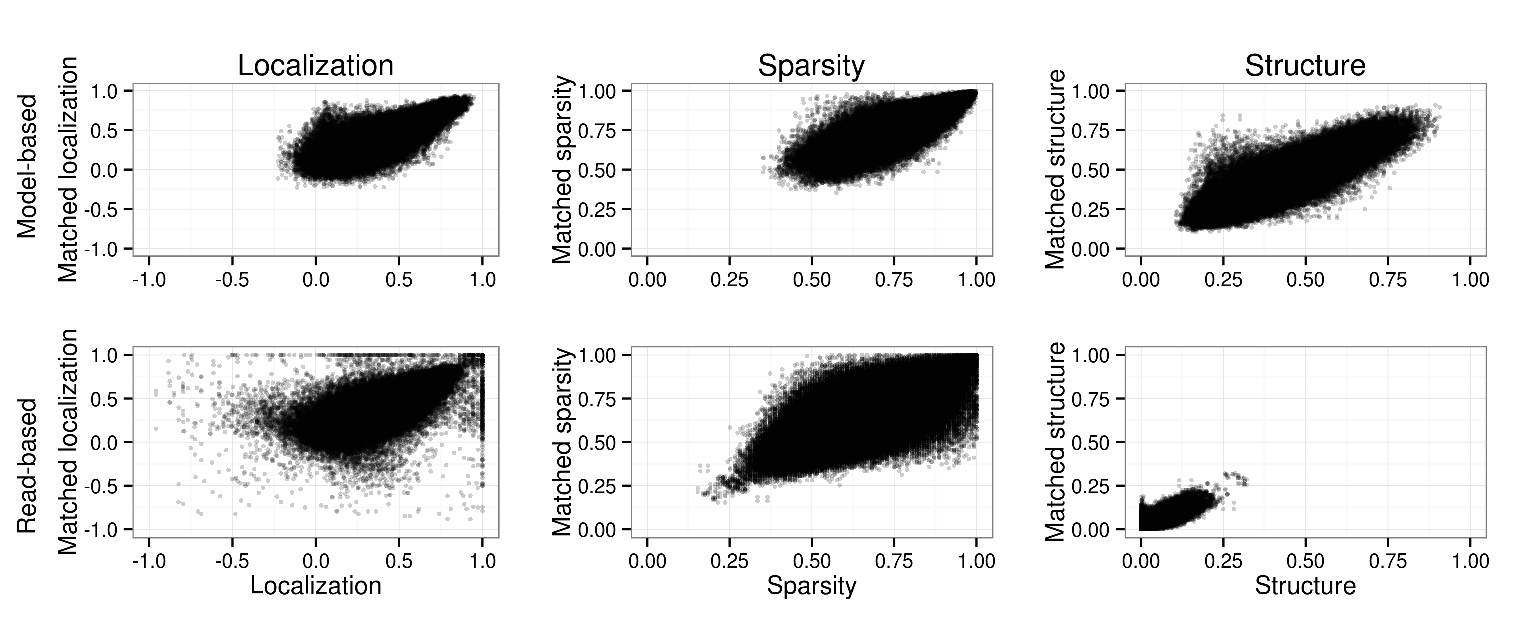
\includegraphics[width=\textwidth]{figures/nucleosomes/figure_cluster_reproducibility_bio}
 \caption{Joint distributions of local, structure, and sparsity indices for matched clusters between biological replicates for model-based (top) and Parzen window/read-based (bottom). \label{fig:clusterReproducibility}}
\end{figure}
\fi

Inferred cluster positions were highly reproducible with a mean best-match distance of $15.72\pm0.14$bp and median best-match distance of 4bp, between biological replicates, and of $14.30\pm0.2$bp and 3bp, respectively, between technical replicates.
With the proposed method, 90\% of clusters were matched within 44bp across biological replicates, and within 35bp across technical replicates.
% EDO : Anything bad happens to the PzW estimator here?
% AWB : No. It does just fine in terms of cluster location reproducibility. Suffers on the cluster-level summaries.
These results are comparable to the those obtained with a Parzen-window estimator, which achieves mean and median best-match distances of $15.24\pm0.14$bp and 4bp, between biological replicates, and of $13.98\pm0.19$bp and 8bp, respectively, between technical replicates.
Inferred cluster positions were also consistent across methods, within each replicate, with mean and median best-match distances of $3.11\pm0.07$bp and 1bp.
Across methods, 90\% of inferred cluster positions were matched within 2bp and 95\% were matched within 3bp.

Cluster-level properties, however, showed significant differences between the model-based and Parzen-window estimates, both in terms of reproducibility and comparability, as Figure \ref{fig:clusterReproducibility} shows.
%
The model-based estimator of the localization estimand $L$
 % EDO : what is this new estimand now? can you refer to an estimand equation or name a specific property (var, st dev) of an estimand?
 % AWB : See first paragraph. All estimators are defined as posterior means of the estimands from 2.3.
 showed the greatest reproducibility with an $R^2$ of $0.765\pm0.002$ between matched clusters for biological replicates ($0.799\pm0.002$ for technical replicates), performing  better than the read-based estimates which had $R^2$'s of $0.713\pm0.003$ and $0.745\pm0.005$, respectively.
%
The model-based estimator of the structure estimand $S$
 % EDO : what is this new estimand now? can you refer to an estimand equation or name a specific property (var, st dev) of an estimand?
 % AWB : See first paragraph. All estimators are defined as posterior means of the estimands from 2.3.
 was close behind with $R^2$'s of $0.749\pm0.002$ and $0.795\pm0.002$ for biological and technical replicates.
However, the read-based estimator of $S$ fared considerably worse with $R^2$'s of only $0.664\pm0.003$ and $0.698\pm0.004$, respectively.
%
The model-based estimator of the sparsity estimand $R$ showed the largest gap in reproducibility between model-based and read-based estimators, with $R^2$'s of $0.720\pm0.002$ and $0.736\pm0.002$ for the model-based method (between biological and technical replicates) and $R^2$'s of only $0.403\pm0.007$ and $0.526\pm0.005$ for the read-based estimator, respectively.

Localization ($L$) was also the most comparable feature between the model-based and read-based estimators with a Spearman correlation of $0.950\pm0.001$ within replicates.
%
This can be seen graphically in the leftmost panels of Figure \ref{fig:clusterReproducibility}: the read-based localization index is noisier than the model-based one, but their distributions appear otherwise comparable.
%
The structure index ($S$) was moderately comparable between the model-based and read-based estimators with a Spearman correlation of $0.784\pm0.001$.
The magnitudes of these estimators are less comparable than the correlation suggests, with the model-based estimator spanning nearly 3 times the range of the read-based one.
%
The sparsity index ($R$) was barely comparable between estimators, as one would expect from the middle panels of Figure \ref{fig:clusterReproducibility}.
Its Spearman correlation was only $0.218\pm0.003$, and the read-based estimator spanned a far wider range of values than the model-based one.
%
These differences arise because the model-based and read-based estimators are actually estimating different quantities.
Read-based estimators are estimating properties of both the experimental errors and the distribution of positions, whereas the model-based estimators are targeting only the underlying distribution of nucleosome positions.

These results show that the proposed methods provide reproducible inferences about the local structure of nucleosome positions across variation from biological and technical sources, including explicit changes to the degree of enzymatic digestion.
They significantly outperform standard Parzen-window and read-based estimators in this regard and provide a richer, more accurate view of the true distribution of nucleosome positions.

\subsubsection{Local concentrations}
\label{sec:detectionReproducibility}

The locations of detected local concentrations (based on $C_{3,147}(k)$) are highly reproducible across both biological and technical replicates.
These results are summarized in Figure \ref{fig:localConcentrationReproducibility}, where we compare the distributions of best-match distances between biological and technical replicates.
%
\ifx\nofigures\undefined
\begin{figure}
 \centering
 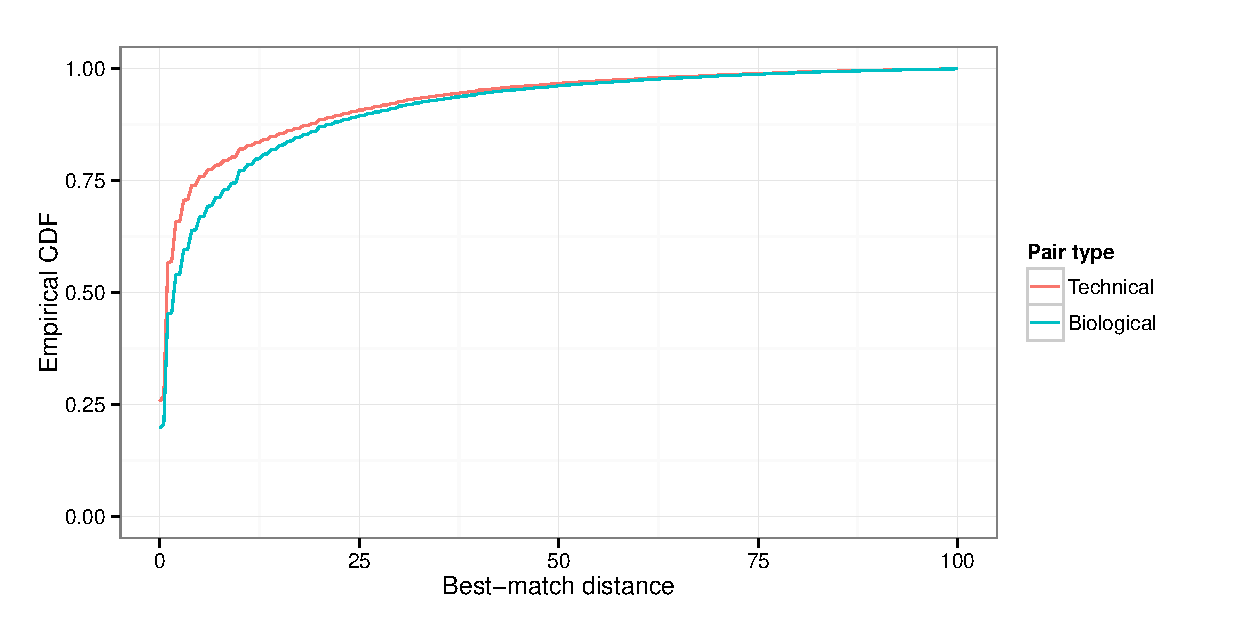
\includegraphics[width=0.8\textwidth]{figures/nucleosomes/plot_reproducibility_cdfs_pm3}
 \caption{Empirical CDFs of best-match distances between detected local concentrations for technical (red) and biological (blue) replicates. \label{fig:localConcentrationReproducibility}}
\end{figure}
\fi

We observe higher reproducibility between technical replicates than between biological replicates, with median best-match distances of 1bp and 2bp, respectively.
%Mean best-match distances were $11.28\pm0.06$bp and $12.77\pm0.04$ bp.
For biological replicates, 75\% of positions were matched within 10bp, 80\% were matched within 15bp, and 90\% were matched within 33bp.
For technical replicates, the corresponding quantiles were 6bp, 11bp, and 30bp.
These results demonstrate the reliability of the proposed method in analyzing high-throughput sequencing data, and provide confidence that the small-scale details of nucleosome positioning identified by the proposed method represent real biological structure.

% Emphasis on follow-up?
% AWB: Edited section 4 up to here

\section{Concluding Remarks}
\label{sec:remarks}

We have presented an approach to modeling and making inferences about the genome-wide distribution of nucleosome positions from paired-end sequencing data.
The results presented in Section \ref{sec:results} demonstrate the utility of the proposed methods for biological analyses, particularly the reproducibility of its inferences across experimental conditions.
Below, we expand on several broader points that have informed the development of these methods, including
 the lack of utility of single-cell constraints in the analyses of measurements on cell populations, 
 the relationship between estimands of interest and the performance gains stemming from model-based inferences on them,
 and the role of distributed computing in inference with massive, high-dimensional data.

\subsection{Modeling}
\label{sec:remarksModeling}

% Independent hierarchical structure; lack of spacing constraints

We explicitly choose not to include prior information on nucleosome spacing in this model.
Previous work has used the empirically-observed 150-200bp spacing between nucleosomes within individual cells to constrain inferences on nucleosome positions \citep[e.g., see][]{Shivaswamy2008,Yuan2005}.
In the presence of alternative nucleosome positioning and chromatin dynamics, however, constraints on spacing that hold on a single-cell level need not hold after aggregation across a population of cells, which is where measurements are taken.
%
With sequencing coverage on the order of 10--100, only a tiny fraction of the cells in the population contribute to the observed data within each small region of the genome.
The probability of observing even two reads from the same cell within, for instance, a single ORF is minuscule.
As a result, single-cell constraints provide few constraints on the range of probable observations in high-throughput sequencing experiments.
%
Thus, the proposed model does not use information on expected separation among nucleosomes along the sequence to constrain the inferred nucleosome positions.
Instead, we opt for a simpler hierarchical structure within each segment, modeling locally shared distributions of nucleosome localization.

% Single-end extensions

The proposed method uses information about the fragment lengths between by pairs of reads that is provided by paired-end sequencing technology to infer the effects of enzymatic digestion on the measurements $\bm{y}$.
Many studies, however, use single-end sequencing technology, which does not provide fragment lengths.
In related work \citep{Xu:Alex:Edo:Erin:2011}, we have developed an approach to estimate the digestion variability template, $\bm t$, for single-end data using an alternative source of fragment-length information; Bioanalyzer technology \citep[e.g.,][]{Mueller2000}.
The model and inference presented in Sections \ref{sec:model} and \ref{sec:estimation} can be adapted to this single-end context with an appropriate modification of the template $\bm t$ and of the digestion matrix $X$.

\subsection{Estimands}
\label{sec:remarksEstimands}

In defining the estimands of biological interest, we aimed at separating properties of the distribution of observed reads, which include the effects of enzymatic digestion, PCR, and sequencing, from  the distribution of nucleosome positions, which is the true target of biological investigations.
Existing estimators defined directly as functions of the read counts confound these distributions, impairing reproducibility of the analysis and ultimately their utility for scientific exploration.
In the model introduced in Section \ref{sec:model}, the distribution of nucleosome positions corresponds to the $\bm \beta$ vector, while the template $\bm{t}$ and the remaining error structure capture other sources of experimental variation.
The estimands presented in Section \ref{sec:estimands} are functions only of the true underlying $\bm \beta$, and are thus unaffected by variation due to the experimental process, at least in principle.
Below, we discuss two subtle points on the construction of these estimands.

First, there is a key distinction between cluster-based estimands such as $L_{i,j}$, $S_{i,j}$, and $R_{i,j,q}$ and other summaries of local structure, such as those based on $C_{p,l}(k)$.
Cluster-based estimands capture the properties of the distribution of nucleosome positions within small regions identified by a clustering algorithm.
%; they include estimands of localization $L$, structure $S$, and sparsity measures $R$.
These measured depend on the particular definition of ``cluster'' and on the clustering method used.
The sensitivity of these estimands to these choices is problematic, in practice, and fine-grained structure is lost in the reduction of data to clusters.
However, this reduction can simplify subsequent interpretation.
%
In contrast, estimands such as the local concentration index $C_{p,l}(k)$ summarize the local structure of the nucleosome position distribution without relying on a clustering criterion.
They lead to reproducible analyses and can be relied upon for scientific discovery of small-scale features.
%
We believe that these classes of estimands are most useful in combination, providing complementary views on the distribution of nucleosome positions.

Second, 
 we have found that the magnitude of the performance gains stemming from model-based inferences depends strongly on the estimand of interest.
%
For instance, the proposed method outperforms read-based estimators in terms of power and error when targeting our cluster-level localization estimands $L$, but the difference in reproducibility is not overwhelming.
However, the increase in reproducibility one can expect from the proposed method is substantial when targeting structure and sparsity measures, $S$ and $R$.
This reflects the greater sensitivity of read-based estimators of structure and sparsity to observation noise.
%
In addition, as we have shown in Section \ref{sec:localPower} and \ref{sec:detectionReproducibility}, the proposed method can  provide  reproducible inferences about individual local features less than 10bp wide, when inference on properties of the distribution of nucleosome positions at such a fine resolution has been so far considered infeasible with read-based estimators.
%
More generally, the more sensitive an estimand is to observation noise, the greater the performance gains expected from using the proposed method.

Our results suggest that careful probabilistic modeling of the core sources of experimental variation can enable new types of scientific inferences.

\subsection{Inference}
\label{sec:remarksInference}

% Scalable MCMC and distributed computation

The use of distributed computing was essential for our method, as it allowed us to sample from the marginal posterior of $\bm \beta$ in only minutes per chromosome.
We leveraged the conditional independence structure of our model to create an efficient, scalable distributed MCMC sampler.
This structure stems from the finite length of the digestion variability template $\bm t$.
As the template is $2w + 1$ wide, subvectors of $\bm \beta$ separated by at least $2w$ base pairs are conditionally independent \emph{a posteriori} given $(\bm \mu, \bm \sigma^2)$.
Thus we can update collections of such subvectors independently across hundreds of processors.
The communication costs involved in this procedure are low, as only each  subvector (padded by $w$ entries on each end) and the relevant entries of $(\bm \mu, \bm \sigma^2)$ are needed for each update.

To update each subvector of $\bm \beta$ in our MCMC, we use a simple HMC step.
Because of the convolution structure of $X$, computation of the conditional posterior and its gradient for $B$-entries-long subvectors of $\bm \beta$ scale as $O(B \log B)$. 
For a fixed block size $B$, adding processors in proportion to the length of the chromosome being analyzed maintains constant runtime.
In addition, the proposed method has constant runtime with respect to the number of fragments observed, omitting alignment.
As shown in Section \ref{sec:mcmcPerformance}, this scalable inference strategy leads to a high-quality sampler.

% Detection; calibrated Bayesian approach

We propose a combination of Bayesian and frequentist techniques for the detection of local concentrations of nucleosomes.
We use the local concentration estimands, $C_{p,l}(k)$, to define the structure of interest.
We then use draws from the parallel HMC sampler to estimate the posterior probabilities of these estimands exceeding their expected value under a locally uniform distribution of nucleosome positions.
%
Instead of using these estimated posterior probabilities to make inferences directly, we calibrate them using frequentist multiple testing techniques \citep{StoreyTibshirani2003}.
Instead of relying upon the model to provide a null distribution for such calibration, we adopt a data-dependent permutation null in the spirit of Fisher's exact test.
%
The calibration step provides guarantees on the behavior of the detection procedure under a permutation null and transforms our Bayesian posterior probabilities to the more standard, interpretable scale of FDRs and q-values.
% and maps our posterior probabilities to a more useful scale of evidence. % EDO : this last remark is cryptic. what scale?
% AWB : Bayesian posterior probabilities with a weakly informative prior have no direct interpretation as either a degree of belief or as a frequency statement. Frequency calibration transforms them to a standard scale (in this case, FDR and q-values).

The pragmatic approach to detection described above is one step in our broader approach to the analysis of nucleosome positioning.
%
First, we used a probability model to build statistics that directly target the scientific estimands of interest, and performed inference with MCMC.
Second, we used permutations to define a reference distribution based on the observed data and the segmentation, and detect local concentrations of nucleosome positions.
Third, we evaluated the power, accuracy, and reproducibility of inferences from our method using biologically-motivated simulations, and technical and biological replicates.
Each step in this strategy reflects less reliance upon modeling assumptions and a greater emphasis on external validity.
%
The success of this strategy is reflected in the empirical results and simulation studies presented in Section \ref{sec:results}.
We obtain accurate, reproducible, scalable inferences about the genome-wide distribution of nucleosome positions with well-studied operating characteristics, providing new capabilities to this area of biology.

